% !TEX TS-program = pdflatex
% !TEX encoding = UTF-8 Unicode

% This is a simple template for a LaTeX document using the "article" class.
% See "book", "report", "letter" for other types of document.

\documentclass[11pt]{book} % use larger type; default would be 10pt
\raggedright


\usepackage[utf8]{inputenc} % set input encoding (not needed with XeLaTeX)

%%% Examples of Article customizations
% These packages are optional, depending whether you want the features they provide.
% See the LaTeX Companion or other references for full information.

%%% PAGE DIMENSIONS
\usepackage{geometry} % to change the page dimensions
\geometry{letterpaper} % or letterpaper (US) or a5paper or....
% \geometry{margin=2in} % for example, change the margins to 2 inches all round
% \geometry{landscape} % set up the page for landscape
%   read geometry.pdf for detailed page layout information

\usepackage{graphicx} % support the \includegraphics command and options
%\usepackage{svg-inkscape}
%\usepackage{svg}
\usepackage{bussproofs}

 \usepackage[parfill]{parskip} % Activate to begin paragraphs with an empty line rather than an indent

%%% PACKAGES
\usepackage{booktabs} % for much better looking tables
\usepackage{array} % for better arrays (eg matrices) in maths
\usepackage{paralist} % very flexible & customisable lists (eg. enumerate/itemize, etc.)
\usepackage{verbatim} % adds environment for commenting out blocks of text & for better verbatim
\usepackage{subfig} % make it possible to include more than one captioned figure/table in a single float
% These packages are all incorporated in the memoir class to one degree or another...

% Packages needed to set discrete math symbols 
\usepackage {amsfonts} % gives mathbb
\usepackage {amssymb}  % gives nmid (does not divide)
\usepackage {amsmath}  % to get text in math mode
\usepackage {amsthm}

% Packages to improve formatting
\usepackage {enumitem}

%% Theorems, Definitions, Corrolaries, etc
\theoremstyle {definition}
\newtheorem {definition}{Definition}[section]
\newtheorem {theorem}{Theorem}[section]
\newtheorem {corollary}{Corollary}[section]
\newtheorem{lemma}{Lemma}[section]

\theoremstyle {remark}
\newtheorem*{notes}{Notes}

%% Graphics, Illustrations, etc
\usepackage {graphics}
\graphicspath{ {illustrations/} }

%%% HEADERS & FOOTERS
\usepackage{fancyhdr} % This should be set AFTER setting up the page geometry
\pagestyle{fancy} % options: empty , plain , fancy
\renewcommand{\headrulewidth}{0pt} % customise the layout...
\lhead{}\chead{}\rhead{}
\lfoot{}\cfoot{\thepage}\rfoot{}

%%% SECTION TITLE APPEARANCE
\usepackage{sectsty}
\allsectionsfont{\sffamily\mdseries\upshape} % (See the fntguide.pdf for font help)
% (This matches ConTeXt defaults)

%%% ToC (table of contents) APPEARANCE
\usepackage[nottoc,notlof,notlot]{tocbibind} % Put the bibliography in the ToC
\usepackage[titles,subfigure]{tocloft} % Alter the style of the Table of Contents
\renewcommand{\cftsecfont}{\rmfamily\mdseries\upshape}
\renewcommand{\cftsecpagefont}{\rmfamily\mdseries\upshape} % No bold!

%%% END Article customizations

%%% The "real" document content comes below...

\title{A Brief Outline of Discrete Mathematics for the Undergraduate Computer Science Student}
\author{Dale Fletter}
\date{\today} % Activate to display a given date or no date (if empty),
         % otherwise the current date is printed 







\begin{document}

\frontmatter        
        \maketitle
        copyright Dale Fletter, 2018
        created using \LaTeX\ 
        %%%%%%%%%%%%%%%%%%%%%%%%%%%%%%%%%%%%%%%%%%
% Formal Book Title Page
% LaTeX Template
% Version 2.0 (23/7/17)
%
% This template was downloaded from:
% http://www.LaTeXTemplates.com
%
% Original author:
% Peter Wilson (herries.press@earthlink.net) with modifications by:
% Vel (vel@latextemplates.com)
%
% License:
% CC BY-NC-SA 3.0 (http://creativecommons.org/licenses/by-nc-sa/3.0/)
% 
% This template can be used in one of two ways:
%
% 1) Content can be added at the end of this file just before the \end{document}
% to use this title page as the starting point for your document.
%
% 2) Alternatively, if you already have a document which you wish to add this
% title page to, copy everything between the \begin{document} and
% \end{document} and paste it where you would like the title page in your
% document. You will then need to insert the packages and document 
% configurations into your document carefully making sure you are not loading
% the same package twice and that there are no clashes.
%
%%%%%%%%%%%%%%%%%%%%%%%%%%%%%%%%%%%%%%%%%



%----------------------------------------------------------------------------------------
%	TITLE PAGE
%----------------------------------------------------------------------------------------


\begin{titlepage} % Suppresses headers and footers on the title page

	\centering % Centre everything on the title page
	
	\scshape % Use small caps for all text on the title page
	
	\vspace*{\baselineskip} % White space at the top of the page
	
	%------------------------------------------------
	%	Title
	%------------------------------------------------
	
	\rule{\textwidth}{1.6pt}\vspace*{-\baselineskip}\vspace*{2pt} % Thick horizontal rule
	\rule{\textwidth}{0.4pt} % Thin horizontal rule
	
	\vspace{0.75\baselineskip} % Whitespace above the title
	
	{\LARGE A BRIEF OUTLINE\\ OF\\  ~DISCRETE MATHEMATICS\\} % Title
	
	\vspace{0.75\baselineskip} % Whitespace below the title
	
	\rule{\textwidth}{0.4pt}\vspace*{-\baselineskip}\vspace{3.2pt} % Thin horizontal rule
	\rule{\textwidth}{1.6pt} % Thick horizontal rule
	
	\vspace{2\baselineskip} % Whitespace after the title block
	
	%------------------------------------------------
	%	Subtitle
	%------------------------------------------------
	
	A Short Course in Discrete Mathematics for a Computer Science Undergraduate % Subtitle or further description
	
	\vspace*{3\baselineskip} % Whitespace under the subtitle
	
	%------------------------------------------------
	%	Editor(s)
	%------------------------------------------------
	
	Edited By
	
	\vspace{0.5\baselineskip} % Whitespace before the editors
	
	{\scshape\Large Dale Fletter \\ D P \\} % Editor list
	
	\vspace{0.5\baselineskip} % Whitespace below the editor list
	
	\textit{The University of California \\ Davis} % Editor affiliation
	
	\vfill % Whitespace between editor names and publisher logo
	
	%------------------------------------------------
	%	Publisher
	%------------------------------------------------
	
	\plogo % Publisher logo
	
	\vspace{0.3\baselineskip} % Whitespace under the publisher logo
	
	2019 % Publication year
	
	{\large publisher} % Publisher

\end{titlepage}

%----------------------------------------------------------------------------------------


% that contains    \begin{titlepage}...\end{titlepage}
        %
        copyright Dale Fletter, 2018\\
        \vspace{1in}
               
       \noindent\rule{8cm}{0.4pt}

        created using \LaTeX\  via TexWorks
        © 2007-2017 Jonathan Kew, Stefan Löffler, Charlie Sharpsteen
       Version 0.6.2 (travis-ci) [r.7ecce17, 4/29/17 9:23 AM]running on a MacBook Pro under macOS Mojave, 10.14.2
       \vspace{1in}
       
       
       Für alle, die die Schönheit von Wissenschaft anderen zeigen wollen.
       
       
       
       
       \noindent\rule{8cm}{0.4pt}
	% that contains copyright, ISBN, etc.
        %\input{dedication}% saying "this book is created for my parents..." 
        %\input{Target Audience}
        %\input{author}% about the author
        %\input{editor}% about the editor
        \setcounter{tocdepth}{1}
        \tableofcontents
        %\listoffigures
        %\listoftables
        %\lstlistoflistings
        



\newpage
 



\chapter {Introduction}
Discrete math is a survey of many different areas of mathematics not covered by the usual series of calculus classes required of an engineering student. Since it is a survey it uses an overwhelming number of conventional symbols that have been adopted over the centuries by mathematicians. You will be reading a paper that was set using a popular free typesetting tool called Latex that is nearly universally used by scientists, engineers and mathematicians to publish papers. At times in this paper you will see references to backslashed sequences like $\forall$, $\in$, etc. These are references to the plaintext markups that are used in Latex in case you want to begin using that tool. For anyone who aspires to graduate school it is a requirement.


While the intent of this material is to be as purely formal as possible, it is necessary to make the course easier to make some assumptions of prior knowledge even before it is formally introduced. For example the section on logic assumes the reader is already familiar with all secondary school math including the concepts of integer versus real numbers and the basic rules of algebra.

\mainmatter

\newpage


                         %%%   LOGIC   %%%
\chapter {Logic}
Logic is foundational for all of science and math. For computer science it is important to recall that most computers are logic machines. While logic can be studied using language you will see that we can abstract away the language and deal with a pure symbolic logic and that will be our focus. We will use this symbolic logic to prove things about any domain that can be represented using propositions and predicates.


\section {Propositional Logic}
   \subsection {Propositions}
\begin {definition}
A proposition is a declarative sentence which is true or false, but not both. Also called a statement.
\end {definition}

Note that sentences with ambiguous antecedents are not propositions.

Note that there are two literal values in this logic, one that represents true and the other that represents false. Most commonly T is used for true and F for false.

Note that questions and commands are not propositions.

We use letters to denote \textbf{propositional variables}, to represent individual propositions just as we use variables to represent numerical values. The letters conventionally used for propositions are p,q,r, etc. The \textbf{truth value} of a proposition is true, denoted by the logical literal T, if it is a true proposition, and the truth value of a proposition is false, denoted by F, it it is a false proposition. 

The area of logic that deals with propositions is called the \textbf{propositonal calculus} or \textbf{propositional logic}. 

    \subsection {Compound Propositions}
    \begin {definition}
    A \textbf{compound proposition} is a proposition formed from atomic propositions with logical operators. 
    \end {definition}

Note Schaum's represents an abstract compound proposition P with atomic propositions p,q,r, etc as P(p,q,r,...).

    \subsection {Negation}
    \begin {definition}
    Let $p$ be a proposition. The \textit{negation of p}, denoted by $\lnot p$ (also denoted by $\overline{p}$, is the statement 
\textit{"It is not the case that $p$."}\\
The proposition $\lnot p$ is read "not $p$". The truth value of the negation of $p$,  $\lnot p$, is the opposite of the truth value of $p$.
    \end {definition} 
    
    \begin{table}[htbp]
   \centering
  
   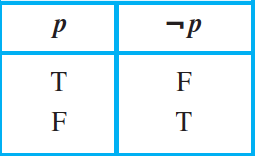
\includegraphics [width=1.5in]{Table-1-1-1-Negation}
   \caption{The Truth Table for the Negation of a Proposition}
   \label{table:negation}
\end{table}
    
    
    
    
    
    Table \ref{table:negation} displays the \textbf{truth table} for the negation of a proposition. A truth table must have a row for each possible combination of true and false values of the propositions used in the compound expression. Note that these rows must be listed in a pattern.

The negation symbol is a unary operator taking the single operand the proposition and giving a new propositon which is the negation of the proposition. 

    \subsection {Conjunction}
\begin {definition} Let $p$ and $q$ be propositions. The \textit{conjuntion} of $p$ and $q$, denoted by $ p \land q$, i the proposition \textit{p and q}. The conjunction $p \land q$ is true when both P and q are true and is false otherwise.
\end {definition}

    \subsection {Disjunction}
Logical disjunction captures part of the meaning of the natural language word "or." But logical disjunction must be carefully observed to have a distinct formal meaning.

\begin {definition}
Let $p$ and q be propositons. The disjunction of P and q, denoted by $p \lor q$, is th eproposition "p or q." The disjunction $p \lor q$ is false when both p and q are false and true otherwise.
\end {definition}

Contrast this with what is called the exclusive or.

\begin {definition}
Let p and q b propsition. Te exclusive or of p and q, denoted by $p \oplus q$, is the proposition that is true when exactly one of p and q is true and is false otherwise.
\end {definition}

Note difference between inclusive and exclusive disjunction.
Note how you can always negate a natural language proposition by prepending the phrase, "it is not the case that..." followed by the original proposition.

    \subsection {Conditional Statements or Logical Implication}

\begin {definition}
Let p and q be propositions. The conditional statement $p \rightarrow $q is the proposition "if p then q" The conditional statement $p \rightarrow q$ is false when p is true and q is false, and true otherwise. In th econditional statement  $p \rightarrow q$, $p$ is called the \textbf{hypothesis} (or \textbf{antecedent} or \textbf{premise})( and $q$ is called the \textbf{conclusion}, \textbf{consequent}.  
\end {definition}

Note: logical implication is not causality. When the antecedent is false the expression is always true. The only way the expression is false is when the antecedent is true and the consequence is false. 
Note: this is a logical operator and must not be confused with the use of the conditional statement in programmng languages.

Conditional statements are a backbone of deductive logic and mathematical reasoning. Yet students often fail to grasp how to understand and use these statements. The lack of understanding here will hamper the ability to avoid many errors in understanding and writing mathematical proofs. 

The conditional statement is also called material implication. In a logic class you will also come across this concept as necessary and sufficient conditions. In logic, the necessary condition is the consequent of the conditional statement. We saw that a material implication is only false when the antecedent is true and the consequent is false. So if we find that the consequent is true and the implication is true, the antecedent MUST BE TRUE. 

Logic also teaches sufficient conditions. The sufficient condition is the antecedent. But having the antecedent be true and the implication be true does not guarantee us that the consequent will also be true. For example, "If you get an A on your final, then you will get an A for the course." Is it necessary for you to get an A on the midterm to get an A in the course? The material implication can still be true even when you got a B on the final, that is you get an A even though it is not the case that you got an A on the final. Getting an A on the final is sufficient for you to get an A in the course but it is not necessary for you to earn an A on the final to get an A for the course.

It will help you if you take the time to understand necessary and sufficient in the context of the material implication.



    \subsection {Inverse, Converse, Contrapositive}
\begin {definition}
Given a conditional statement $p \rightarrow q$, its \textbf{inverse} is the statement $q \rightarrow p$, its converse is $\lnot p \rightarrow \lnot p$ and its \textbf{contrapositive} is the statement $\lnot q \rightarrow \lnot p $
\end {definition}
 

        \subsubsection {The Bi-Conditional}
\begin {definition}
Let $p$ and $q$ be propositions. the \textit{biconditional statement} $p \leftrightarrow q$ is the proposition "$p$ if and only if $q$." The biconditional statement $p \leftrightarrow q$ is true when $p$ and $q$ have the same truth values, an d is false otherwise. Biconditional statements are also called \textit{bi-implicatons}.
 \end {definition}
 Note that you get the same truth values for the compound expressions $p \leftrightarrow q$ and $(p \rightarrow q) \land (q \rightarrow p)$.
 
     \subsection{Precedence of Logical Operators}
Without parentheses compound logical statements can become ambiguous. To avoid a large number of parentheses we adopt a convention of \textbf{operator precedence}. See Table \ref{table:precedenceOfLogicalOperators}.




\begin{table}[htbp]
   \centering
  
   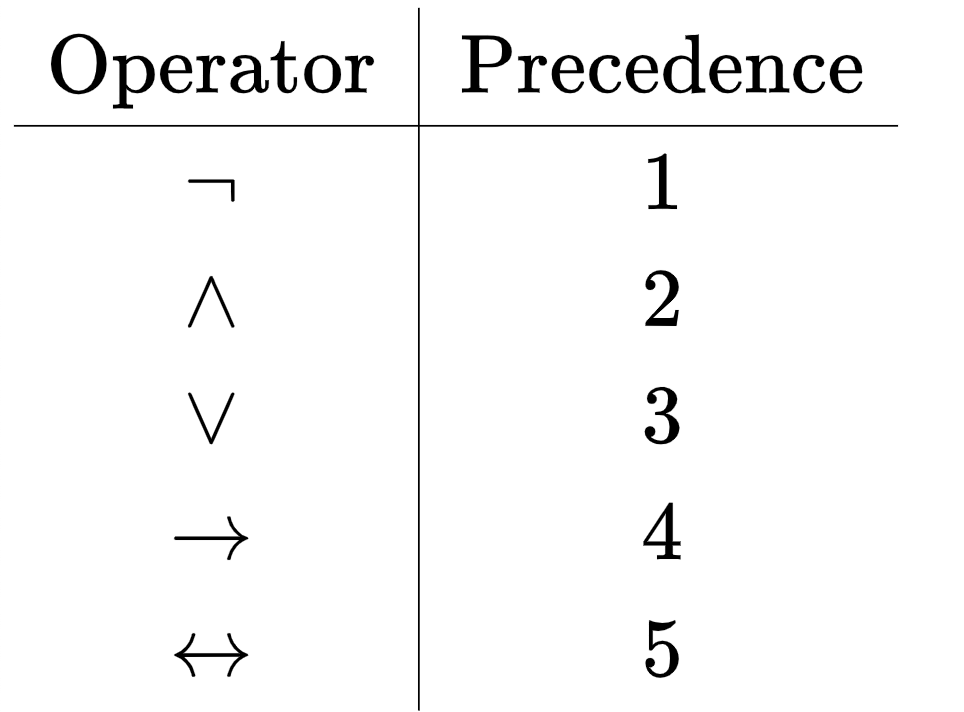
\includegraphics [width=1.5in]{PrecedenceOfLogicalOperators}
   \caption{Precedence of Logical Operators}
   \label{table:precedenceOfLogicalOperators}
\end{table}






     \subsection{Evaluation of Compound Expressions Using Truth Tables}
      Truth Tables can be used to help derive the truth value of complex compound logic statements. Take the innermost binary operations required by the rules of precedence and create a column. Give the truth values for that small compound statement and then build up until you have the entire statement. 

    \subsection {Translating Between English Sentences and Propositional Logic}

    \subsection {System Specification using Symbolic Logic}
consistent statements

    \subsection {Logic and Bit Operations}
bit, Boolean variable, bit operations, 

\begin {definition}
a bit string is a sequence of zero or more bits. The length of this string is the number of bits in the string
bitwise OR, bitwise AND, bitwise XOR.
\end {definition}
The compound proposition $p \land \lnot p$ is a contradiction while the proposition $p \lor \not p$ is a tautology.




\section {Propositional Equivalences}

\begin {definition}
A compound proposition that is always true , no matter what the truth value of the poisitons that occur in it, is called a \textit{tautology}. A compound proposition that is always false is called a \textit{contradiction}. A compound proposition that is neither a tautology nor a contradiction is called a \textit{contingency}.
\end {definition}

    \subsection {Logical Equivalences}
\begin {definition}
The compound proposition $p$ and $q$ are called \textit{logically equivalent} if $p \leftrightarrow q$ is  tautology. The notation $p \equiv q$ denotes that $p$ and $q$ are logically equivalent.
\end {definition}

Note: The symbol $\equiv$ is not a logical connective and $p \equiv q$ is not a compound proposition but a statement that $p \leftrightarrow q$ is a tautology. 

Two distinct propositions may evaluate to the same truth value for each combination of the atomic truth values. These two propositions are said to be logically equivalent or simply equivalent. This can be shown with a truth table and constitutes a valid proof of the equivalence.

\begin{table}[htbp]
   \centering
   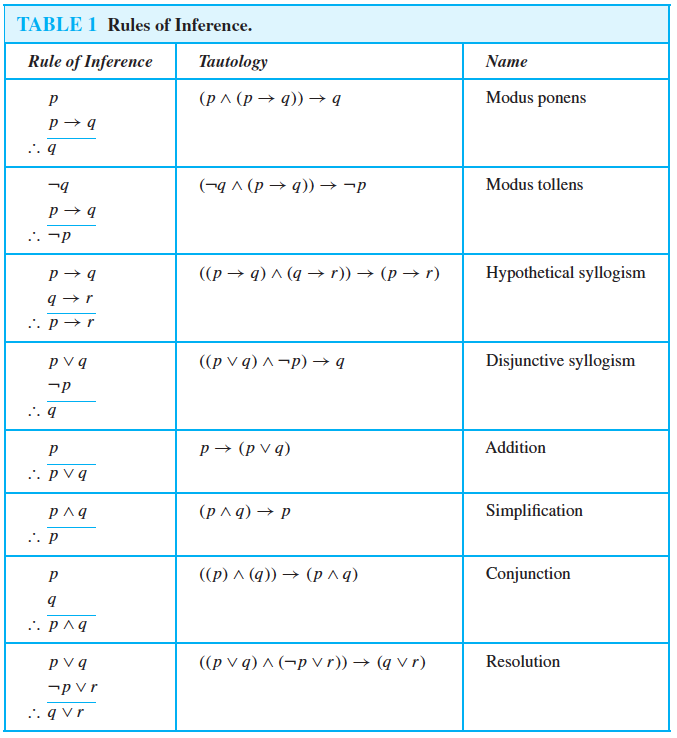
\includegraphics [width=5in] {Table-1-6-1-RulesOfInference}
   \caption{Common Rules of Inference}
   \label{table:rulesofinference}
\end{table}

  \begin{table}[htbp]
  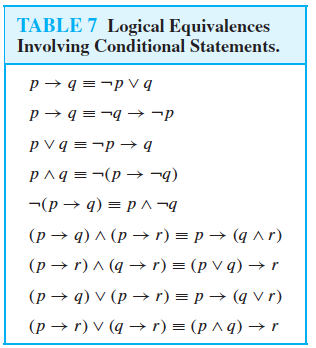
\includegraphics [width=3in]{Table-1-6-7-LogicalEquivalencesInvolvingConditionalStatements}
  \caption{Logical Equivalences Involving Conditional Statements}
  \label{table:logicalequivalencesinvolvingconditionalstatements}
  \end{table}
  
  
  \begin{table}[htbp]
  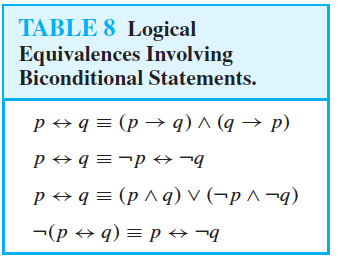
\includegraphics [width=3in]{Table-1-6-8-LogicalEquivalencesInvolvingBiconditonalStatements}
  \caption{Logical Equivalences Involving Bi-Conditional Statements}
  \label{table:LogicalEquivalenceInvolvingBiconditionalStatements}
  \end{table}


    \subsection {Propositional Satisfiability}
\begin{definition}
A compound proposition is \textbf{satisfiable} if there is an assignment of truth values to the variables in the compound proposition that makes the statement form true.
\end{definition}





\section {Predicates and Quantifiers}
Predicate Logic. First order logic. There are other higher order logics. 
Propositional logic, zero order logic, cannot help with obviously true statements like, "Socrates is a man, all men are mortal, therefore Socrates is mortal". We need to introduce a way to prove such truths. This is called Predicate Logic or Predicate Calculus.

    \subsection {Predicates}
Some objects can have a property. A person may be tall or short. A number may be greater than 100. When we use variables to represent these objects we need a way to test them for the presence or absence of the quality we care about. We call these \textbf{propositional functions} and we call the quality being checked for \textbf{predicates}. 

For example, we may have a variable $x$ which is an integer. We can have a predicate which tests it to see if it is greater than 100. The predicate is "... is greater than 100" and we apply that to the variable $x$.

\begin{definition}
A \textit{predicate} is a function which when applied to an object will evaluate to true when some property is present and false otherwise. We denote the predicate using a capital letter and write the expression using a functional notation. So the predicate $P$ when applied to the variable $x$ is written $P(x)$ and will take on the value of true or false when the value of $x$ has been fixed (bound).

Predicates are not limited to one argument but can have any number of arguments, called \textit{n-place predicates}. For example the predicate $S$ could be "...have the same color" and can accept pieces of fruit as objects. Then the expression $S(p,q,r,s,t)$ will be true if the color of each piece of fruit $p,q,r,s,t$ matches the others and false otherwise.

We often define a predicate using the notation, $P: x+1 > x$.
\end{definition}

\begin{notes}
More advanced texts may discard the parentheses around the arguments in a propositional function
\end{notes}
   \subsection {Quantifiers}
Variables can be bound to values. But we often wish to assert a proposition over a range of values or to claim that there is an object with some property. This process of creating a proposition over some range of objects is called \textit{quantification}. The two fundamental quantifications are the universal and the existential.

        \subsubsection {Universal Quantification}
Many mathematical statements assert that a property is true for all values of a variable in a partiocular doman, called the \textbf{domain of discourse} (or \textbf{universe of discourse}, often just referred to s the \textbf{domain}. Such a statement is expressed using universal quantification. The universal quantification of $P(x)$ for a particular doman in the proposition that asserts that $P(x)$ is true for all values of $x$ in this domain. Note that the domain specifies the possible values of the variable $x$. The meaning of the universal quantification of $P(x)$ changes when we change the domain. The domain must always be specified when a universal quantifier is used; without it, the universal quantification of a statement is not defined.

\begin{definition}[Universal Quantification]
The universal quantification of P(x) is the statement 
$$\text{"}P(x) \text{ for all values of }x \text{ in the domain."}$$
The notation $\forall x P(x)$ denotes the universal quantification of $P(x)$. Here $\forall$ is called the universal quantifier. We read $\forall x P(x)$ as "for all x P(x)" or "for every x P(x)". An element for which $P(x)$ is false is called a counterexample of $\forall x P(x)$.
\end{definition}

\begin{notes}
Generally an implicit assumption is made that all domains of discourse for quantifiers are nonempty. Note that if the domain is empty, then $\forall P(x)$ is true for any propositional function $P(X)$ because there are no elements $x$ in the domain for which $P(x)$ is false. 
\end{notes}


        \subsection {Existential Quantifier}
Many mathematical statements assert that there is an element with a certain property. For example, for any integer $i$ there is another integer $j$ such that $i+j=0$. Such statements are expressed using existential quantification. With existential quantification, we for a proposition that is true if and only if $P(x)$ is true for at least one value of $x$ in the domain.

\begin{definition}
The \textit{existential quantification} of $P(x)$ is the proposition
$$\text{"There exists an element }x \text{ in the domain such that } P(x) \text{ ."}$$
We use the notation $\exists x P(x)$ for the existential quantification of $P(x)$. Here $\exists$ is called the \textbf{existential quantifier}.
The domain must always be specified when a statement $\exists P(x)$ is used. The meaning of $\exists P(x)$ changes when the domain changes. without specifying the domain, the statement $\exists P(x)$ has no meaning. The existential quantifier $\exists P(x)$ is read as, "There is an $x$ such that $P(x)$, "There is at least one $x$ such that $P(x)$", or "For some $x P(x)$".
\end{definition}

\begin{notes}
Generally, an implicit assumption is made that all domains of discourse for quantifiers are nonempty. If the domain is empty, the $\exists P(x)$ is false whenever $P(X)$ is a propositional function because when the domain is empty, there can be no element in the domain for which $P(x)$ is true.
\end{notes}

    \subsection {Other Quantifiers}
You will sometimes see other quantifiers but the only one which occurs often enough to get notice is the uniqueness quantifier:

\begin{definition}
The \textit{uniqueness quantification} of $P(x)$ is the proposition:
$$\text{"There exists exactly one element }x \text{ in the domain such that }P(x)\text{".}$$
We use the notation $\exists !$ for the uniqueness quantification.
\end{definition}
    \subsection {Quantifiers with Restricted Domains}
An abbreviated notation is sometimes used to specify some subset of the domain. For example $\forall x <0 (x^2 >0)$ in the domain of real numbers places the restrictive clause next to the quantifier.

    \subsection {Precedence of Quantifiers}


    \subsection {Binding Variables}
\begin{definition}
When a variable has been assigned a value, we say the value has been \textbf{bound} to the variable. Any variable that has not yet been bound to a value is said to be \textbf{free}. The \textbf{scope} of the binding is controlled by the use of parentheses or other marks. The value of a variable is also bound by the use of a quantifier and the variable is either within or outside the scope of that quantifier.
\end{definition}

    \subsection {Logical Equivalences Involving Quantifiers}
\begin{definition}
Statements involving predicates and quantifier are \textit{logically equivalent} if and only if they have trhe same truth value no matter which predicates are substitued into these staeent and which domain of discourse is used for the variables in these propositionan functions. We use the notation $S \equiv T$ to indicate that two statements $S$ and $T$ involving predicates and quantifiers are logically equivalent.
\end{definition}

    \subsection {Negating Quantified Expressions}
\begin{notes}
$\neg \forall x P(x) \equiv \exists x \neg P(x)$ is a logical equivalence.
\end{notes}
    
    \begin{table}[htbp]
  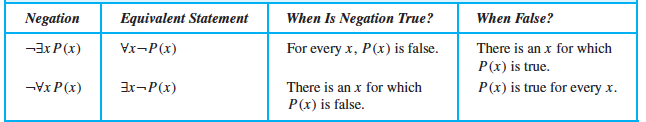
\includegraphics [width=3in]{DeMorgansForQuantifiedExpressions}
  \caption{DeMorgansForQuantifiedExpressions}
  \label{table:DeMorgansForQuantifiedExpressions}
  \end{table}
    

    \subsection {Translating Between English and Quantified Expressions}
    \subsection {Using Quantifiers in System Specification}
    \subsection {Logic Programming}


\section {Nested Quantifiers}
Thinking of Quantification as Loops
    \subsection {The Order of Quantifiers}
\begin{table}[htbp]
  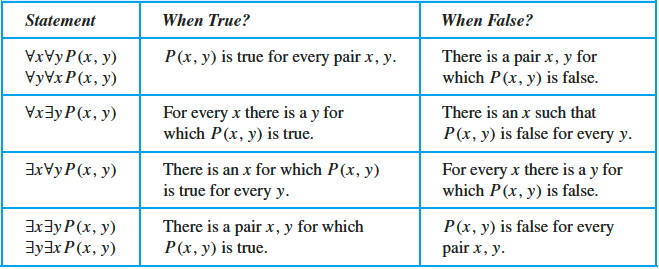
\includegraphics [width=3in]{Table-1-4-1-QuantificationOfTwoVariables}
  \caption{Quantification Of Two Variables}
  \label{table:QuantificationOfTwoVariables}
  \end{table}
    
Table-1-4-1-QuantificationOfTwoVariables
    \subsection {Translating Between English and Nested Quantified Statements}
    \subsection {Negating Nested Quantifiers}


\section {Rules of Inference}
   \subsection {Valid Arguments in Propositional Logic}
   \subsection {Rules of Inference for Propositional Logic}
   \subsection {Using Rules of Inference to Build Arguments}
   \subsection {Resolution}
   \subsection {Fallacies}
   \subsection {Rules of Inference for Quantified Statements}
   
  \begin{table}[htbp]
  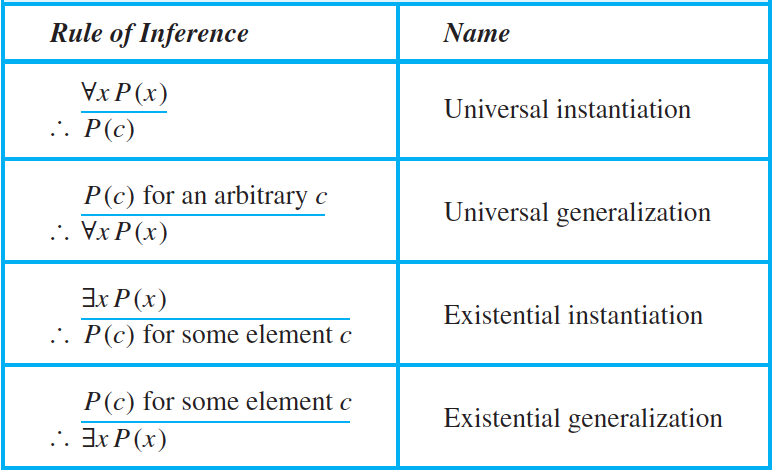
\includegraphics [width=3in]
  {Table-1-6-2-RulesOfInferenceForQuantifiedStatements}
  \caption{RulesOfInferenceForQuantifiedStatements}
  \label{table:RulesOfInferenceForQuantifiedStatements}
  \end{table}
  
  We see that quantified statements need a couple additional rules of inference. They are summarized in Table \ref{table:RulesOfInferenceForQuantifiedStatements}
   
   \subsection {Combining Rules of Inference for Propositions and Quantified Statements}
 
 






         %%%%%%%%%%%%%%%%%   PROOFS   %%%%%%%%%%%%%%%%%%%%
\chapter{Introduction to Proofs}
The last chapter introduced a great deal of terminology and basic logical structure. But many feel that real mathematics, including logic, does not begin until one begins to reason about the material and attempt to determine new truths from the truths that are either accepted as true or which can be arrived at through reason. This chapter is a fast introduction to this mode of reasoning.

The chapter introduces the basic terminology of deductive reasoning and its presentation in the form of formal proofs. Various proof methods and strategies are summarized with classic examples. The remainder of the book will build upon this basis and demonstrate good proof style.

\section {Introduction to Proofs}
  \subsection {Why Write Proofs?}
Mathematics can be distinguished from other scientists by the kind of reasoning that we do. For reasons that this course explains, computer science is mostly a form of applied mathematics and therefore learning how to do mathematical proofs is a needed skill for a true computer scientist. Reasoning is often split into two types, inductive and deductive. Inductive reasoning is that which tries to generalize from a series of observations while deductive uses logic to conclude that an assertion must be true based on other statements that are already accepted as true. When someone gives a series of assertions that each build on what has come before and using accepted reasoning, we say they have proven their assertion and that the argument is a valid proof of the assertion. This has been a part of logic since at least Euclid's geometry and continues to be a cornerstone of undergraduate education. This chapter will be a poor substitute for a full semester course on the subject but should at least prepare the student for more formal work.

  \subsection{What Am I Allowed to Assume for this Proof?}
Given the emphasis on using accepted truths as premises, the student quickly finds themselves asking, what am I allowed to assume as either a premise or a rule of inference? The last chapter gave the most common ones from logic but often the student must use some high school algebra. The simple answer is that anything you could do in high school as valid algebra can be done in a proof for this course. More formally it must be something that can be justified by some argument to authority, which will be some previously published property. And of course it needs to be applied correctly. What cannot be done is to introduce a truth that in any way assumes the conclusion one is trying to make. We deal with that in this chapter when talking about fallacies.


    informal proofs, theorem, propositions, facts, results, proof, axioms, postulates, lemma, corollary, conjecture
    \subsection {Understanding How Theorems Are Stated}
Often there is an \textbf{assertion} we want to make, some \textbf{proposition} which must either be true or false. Assertions often start as \textbf{conjectures}, propositions which we do not yet know are either true or false and which we would like to have a proof but do not yet have one. We often start with basic definitions which are essentially \textbf{axioms} that we accept as true without question. We must then construct a series of statements that each make new assertions by using the prior axioms and the \textbf{accepted rules of inference}. If we are successful, the final assertion is the proposition we wanted to prove which we call the \textbf{conclusion} of the argument. When we are presenting the assertion with the list of infered assertions that lead to the conclusion, we call this a \textbf{proof}. \textbf{Theorems} are nothing more than assertions we find helpful presented with their arguments as to why the assertion must be true. 

It is not uncommon that something accepted as an axiom is later found to be untrue, that is false. Or that a proof which depended upon a prior theorem which is found to contain a flaw. This leads to an important point about proofs, one can present a \textbf{valid} argument, one which uses only valid rules of inference, yet is found to depend upon one or more premises that are false. The argument is still said to be valid but the argument unsound. To be a \textbf{sound} argument one must have valid reasoning plus true premises. 

\section{Proof Styles}
  \subsection{Proof by Truth Table}
If you can show that two statements always have the same truth value regardless of the truth value of the variables in the expression, you have demonstrated logical equivalence and one can always be substituted for the other where ever it appears. This can be done by creating a truth table with each expression at the top of a column and a row for every combination of truth values of the atomic propositions and show that the two columns have the same values on every row. But since the number of rows in a truth table grows exponentially with the number of atomic propositions, this method is only useful for small equivalences.
  \subsection{Two-Column Proofs}
High-school geometry teaches a two-column method. Some algebra classes use a similar approach to evaluating algebraic expressions. Most introductions to proofs begin with this form of proof presentation. Each line is a statement that is derived deductively from the lines above it. This is less tedious than a truth table proof and seems to correspond with how humans can follow detailed logic. In the most rigorous approach each line must list the inference explicitly in the right hand column to justify the statement just made. This has the advantage of making a student carefully understand how they are using logic to make the statements and easier for a grader to see that valid logic has always been applied. But the insistence on listing every rule applied makes the proof tedious for longer proofs as trivial points of logic clutter the work.
  \subsection{Prose Style Proofs}
Traditional mathematicians used a prose style of proof. The best of this technique applies all the rules of non-fiction writing. You make reasonable assumptions of what your reader will easily follow and which leaps of inference require some parenthetic remark to aid the reader. Good proof presentations in this form use natural language in a rigorous way yet will still suffer from an occassional slip  in inference. Yet by the end of the first introduction to proofs this is the way undergrads are expected to present their proofs. The vital point to recall is that any proof in this form could be reduced to a two-column proof if demanded. Experienced graders will look for large leaps and critically examine the inference to see if it is valid. If you feel it is correct but cannot justify it to yourself, take the time to break it into two or more steps that you can see the rule application.
  \subsection{Other Proof Styles}
Machine proofs are an area of research and many more rigorous proof styles have been described in the past 100 years. This is beyond the scope of an introductory proof class but we mention some of the notational forms used to prepare you for more advanced work. 

Note that many proofs are presented in this fashion:

and will use a notation called a turnstile $\vdash$
    
\section {Methods of Proving Theorems}
This section describes the most basic form of proof style which is the direct proof and introduces the language with which we discuss proofs.
    \subsection {Direct Proofs}
In the chapter on Logic, there was a table of logical equivalences, Table \ref{table:LogicalEquivalenceInvolvingBiconditionalStatements}. The equivalence was demonstrated by showing that no matter the truth condition of the propositions, both expressions would evaluate to the same truth value. That is, the truth tables for both columns under the expressions matched on every row. This is a proof by truth table. However the number of rows will grow exponentially with the number of propositions so this kind of proof cannot be done by hand and often not even by machine for large numbers of propositions. 

This leads to the more common style of proof which is the series of statements grounded on the prior truths but making a new and equivalent statement. We stated the rule of inference known as Modus Ponens which says that given a true conditional statement and the fact that the antecedent of the conditional is known to be true, that the consequent of the conditional must be true. 

$$p \land (p \rightarrow q) \equiv q  \text{    (Modus Ponens)}$$
    
    \subsection {Proof by Contraposition}
    indirect proofs, vacuous and trivial proofs
    \subsection {Proofs by Contradiction}
    A proposition must be either true or false (rule of excluded middle). If it can be shown that a proposition cannot be false, then it must be true. To do this assume the opposite of what is to be proven and then show that it leads to a contradiction. Recall that a contradiction is false regardless of the truth values of the propositions. Once this is done you can assert that the contradiction is false and then conclude that the hypothesis must be true.
    \subsection {Mistakes in Proofs}
    begging the question, circular reasoning
    \subsection {Just a Beginning}
  
\section {Proof Methods and Strategy}
    \subsection {Exhaustive Proof and Proof by Cases}
    without loss of generality (WLOG)
    \subsection {Existence Proofs}
    Constructive Existence Proof, Non-constructive Existence Proof
    \subsection {Uniquenes Proofs}
    
    \subsection {Proof Strategies}
    \subsection {Looking for Counterexamples}
    \subsection {Proof Strategy in Action}
    \subsection {Additional Proof Methods}

\section{Formal Methods}
An important application of proof techniques is found in the study of what is called formal methods which includes proofs of program correctness


  \subsection {Program Verification}A program is said to be correcrt if it produces the correct output for every possible input. A proof of correctness for a program consists of two parts. The first part shows that the correct answer is obtained if the program terminates. This part is said to establish the partial correctness of the program. The second part proves that the program always terminates. When working with proofs of program correctness we use two propositions. The first, called the pre-conditions, gives a proposition that all input values must satisfy. In addition the second proposition is called the post-condition and if the program has correctly computed the value it will evaluate to true. The pre- and post-conditions are sometimes called the initial and final assertions.

\begin{definition}
A program, or program segment, $S$ is said to be partially correct with respect to the initial assertion $p$ and the final assertion $q$ if whenever $p$ is true for the input values of $S$ and $S$ terminates, then $q$ is true for the ouptut values of $S$. The notation $p[S]q$ indicates that the program, or program segment, $S$ is partially correct with respect to the initial assertion $p$ and the final assertion $q$. The notation $p[S]q$ is known as a \textit{Hoare triple}.
\end{definition}

  \subsection {Rules of Inference}
composition rule
  \subsection {Conditional Statements}
  \subsection {Loop Invariants}
        
\newpage


\section {Proofs-redacted}
  \subsection {Rules of Inference for Propositonal Logic}
law of detachment, modus ponens, 
Table: Common Rules of Inference
  \subsection {Using Rules of inference to Build Arguments}
  \subsection {Resolution}
  \subsection {Fallacies}
fallacy of affirming the conclusion
fallacy of denying the hypothesis
  \subsection {Rules of Inference for Quantified Statements}
Universal Instationtiation
Universal Generalization
Existential instantiation
Existential generalization
Table: Rules of Inference for Quantified Statements
  \subsection {Combining Rules of Inference for Propositions and Quantified Statements}
universal modus ponens
universal modus tollens




informal proofs, theorems, axioms, postulates
lemma, corollary, conjecture 
    \subsection {Understanding How Theorems are Stated}
    \subsection {Methods of Proving Theorems}
    \subsection {Direct Proofs}
    \subsection {Deductive Proof Techniques}
Proofs can be divided into two categories, Deductive and Inductive. We present deductive proofs here and save inductive proofs for the chapter on Integers.

Many properties of mathematics are stated If x then y. This is a simple conditional statement and we know from the truth table that the CONDITIONAL STATEMENT will be true in all cases EXCEPT when the antecedent is true and the consequent is false. This makes it easy to prove since we can assume the antecedent is true (why) and then show through a series of logical steps that the consequent must follow from the antecedent. 

The easiest, yet most difficult to grasp initially, is the vacuous proof. The logic is that if there is no member from the domain which can satisfy the conditional statement, the implication is always true. This comes up frequently in edge cases.
 
\subsection {Direct Proofs}
\begin {theorem}
The sum of two even numbers is even
\end {theorem}
Proof (direct proof):

\begin {definition}
an even number can be expressed as 2*some integer
\end {definition}

\begin {definition}
an odd number can be expressed as 2*some integer plus 1
\end {definition}

Let n,m be the two even numbers (premise given)
Then n=2*k and m=2*j where k and j are integers (def of even)
Then n+m=2*k + 2*j (basic law of arithmetic)
Then n+m=2*(k+j) (associative law of arithmetic)
Then n+m is even (def of even)    QED

\subsection {Indirect Proof: Proof Using Contraposition}
Many proofs can be difficult to prove directly. But sometimes they are easier to prove using the contrapositive statement of the proof. This is just one common example of what is called an indirect proof. Recall that the contrapositive is the logical equivalent of any conditional statement. If you can prove the contrapositive, you have proven the conditional.

\subsection {Indirect Proof: Proof by Contradiction}
Not all proofs are given in the form of a conditional. Sometimes it is a direct assertion. Sometimes these statements can be proven using a technique called proof by contradiction or reducto absurdum. Do not confuse this with contrapositive. A contrapositive is the proof of a conditional statement while proof by contradiction is usually not. Proof by contradiction depends upon some basic truths of logic. A proposition must be either true or false, there is no other choice. This is called the law of the excluded middle. So if you can show that a statement MUST be false, then it must be true. How do you show that a statement must be false? If the statement can be restated as a contradiction, then it is false. 

The most famous example of a proof by contradiction is that the square root of 2 is irrational.

\begin {definition}
a rational number is one that can be expressed as the division of two integers
\end {definition}

\begin {definition}
all numbers that cannot be expressed as rational are irrational
\end {definition}

\begin {theorem}
The square root of 2 is irrational
\end {theorem}

Proof (by contradiction)
Assume the square root of 2 is NOT irrational.
Then the square root of 2 would be rational
Then the square root of 2 could be expressed as the quotient of two integers.
Let the square root of 2 be expressed as the rational number n/m (def rational)
Then m*root 2 = n
Then m**2 * 2 = n**2
???
    Note the logical equivalence of the conditional and the expression using only negation and either conjunction or disjunction.

Using the rule of substitution, we can use the rules of equivalence to give us an algebra of propositional logic. Any equivalence rule gives us an alternative way to write the expression that preserves the truth value. Note that in a truth table any two propositions will have identical columns in a truth table. In general while a truth table can be used to show equivalence, once you have more than 4 atomic propositions proving that two expressions are equivalent is more easily done with algebra than with truth tables.

argument: a set of propositions (premises) that is asserted to result in another proposition (conclusion). We formalize this to "prove" things. We say that an argument is valid when the conclusion is true whenever all the premises are true. An argument which is not valid is said to be a fallacy. A valid argument where all the premises are true is said to be sound.

We can write this in two ways:
Let P1, P2, P3, etc be a set of axioms and let Q be the conclusion

sentential, and this is equivalent to the logical statement
$P1 ^ P2 ^ P3^ ... |- Q$
and sometimes it is written as P1, P2, P3, ... |- Q where the conjunction is understood.

or 

P1
P2
P3
(underline)
therefore Q
QED

QED is short for Quod Erat Demonstrandum which means "that which was to be demonstrated. In typeset material the QED is often replaced with a black square.

There are a set of arguments that are used so often they have been given names. For example 

p, p -> q, |- q 

is known as Modes Ponens. These common arguments are summarized in Table 1.2: Rules of Inference. Note you are always free to create a new rule of equivalence.

Modus Ponens
Modus Tolens

Proof
A proof is an argument such that it accepts a certain number of propositions (axioms) which are taken to be true and using valid rules of inference and rules of equivalence results in stating the conclusion. To be a valid proof each line in the proof must be either an axiom or it must be supported by some rule of equivalence or inference. All students begin writing proofs by exhaustively showing the rules they used in a line-by-line format. But as you become more sophisticated you are allowed to skip steps that you assume the reader can follow. However if challenged you must always be prepared to give the step-by-step explanation of the reasoning.


What Can You Assume in Writing a Proof?
Students new to the formalism of mathematics can become confused as to what logical steps do not need support. In general for this class you can assume that everything you learned in secondary school can be used without support. Within a week (for the summer session) you can begin to drop the simplest logical steps and combine them. If there is doubt that the reader (your grader) will be able to see the steps you took to get to your conclusion, it is always ok to over simplify. And if you are unsure of the steps, it is always helpful to over simplify since the grader can point to the specific step you took which was invalid.

other ways are called indirect proofs
    \subsection {Proof by Contraposition}
        \subsubsection {Vacuous and Trivial Proofs}
 
\subsection {Proof Methods and Strategy}
  \subsection {Exhaustive Proof and Proof by Cases}
  \subsection {Existence Proofs}
  \subsection {Uniqueness Proofs}
  \subsection {Proof Strategies}
  \subsection {Looking for Counterexamples}




                          %%% SETS %%%
\chapter {Sets}

\section {Set Definition}
%This is only an introduction to set theory as originally presented by Georg Cantor, now known as naive set theory to set it apart from later work which attempts to put it onto an axiomatic basis. 

\begin {definition}
A \textit{set} is an unordered but well defined collection of objects which are called the \textit{elements/members} of the set.  The objects in a set are called the \textit{elements} or \textit{members}, of the set. A set is said to \textit{contain} its elements. We write $a \in A$ and say, ``a is an element of the set A'' to mean that $A$ contains $a$ and $a \notin A$ to mean that the element $a$ is not contained by the set $A$.
\end {definition}

\begin{notes}
   Sets are unordered. \{a, b\} is the same as \{b, a\}. The number of times an object is enumerated makes no difference, it is still one element.
\end{notes}


  \section{Set Specification}
    \subsection {Set Enumeration}
  The easiest way to describe small sets is to enumerate (list) the elements. This is done by writing the elements between braces with a comma between them. For example let $V$ be the set of English vowels. We can write $V=\{a,e,i,o,u\}$ to define the set $V$. If we want to talk about the positive odd integers less than 10 as the set $O$, we can define it as the set $\{1,3,5,7,9\}$. 
The set $M=\{1, "1", \text{my dog Rover}, \text{red-head}\}$ can be a set. The notation $a_1,a_2,a_3 \in A$ is the same as $a_1 \in A, a_2 \in A, a_3 \in A$. We can start a pattern and use the ellipses symbol to indicate that the reader should infer the pattern. R=\{3,6,9,12,15, \dots\}. $\{0,1,2,3, \dots ,100\}$ The enumeration can be a description of the elements. \{addresses on Pine Street\} defines a set of addresses that are on Pine Street. $O=\{ \text{positive odd integers less than 10} \}$. 


     \subsection {Set Builder Notation}
Set comprehension, set intension. Three parts, a variable, a colon or vertical bar and a logical predicate.  


$\{a | \text{  a is a positive integer }\} $

or 

$E: \text{is even}$, 
$A= \{a | E(a)\}$\\
We read this as 
set A is defined as the set of all $a$ such that $a$ is even. The vertical bar is read "such that". To the left are the variables that represent the set members and to the right is the condition that all members must satisfy.

Example: $A = \{x | \lnot E(x),x<10\}  $

\begin{notes}
Predicates separated by commas are implied conjunction.
\end{notes}
  
Sometimes we restrict the domain of a quantified statement explicitly by making use of a particular notation. For example, $\forall x \in S (P(x))$       %∀x∈S(P(x)) 
denotes the universal quantification of $P(x)$ over all elements in the set $S$. In other words, $\forall x \in S (P(x))$  is shorthand for $\forall x (x \in S(P(x)) \rightarrow P(x))$    
%∀x∈S(P(x)) is shorthand for ∀x(x ∈ S → P(x)).
Similarly, $\exists x \in S(P(x))$ denotes the existential quantification of $P(x)$ over all elements in $S$. That is, $\exists x \in S(P(x))$ is shorthand for $\exists x (x \in S \land P(x))$.
%Similarly, ∃x∈S(P(x)) denotes the existential quantification of P(x) over all elements in S.
%That is, ∃x∈S(P(x)) is shorthand for ∃x(x ∈ S ∧ P(x)).


\section {Common sets and their Notation in Mathematics and Computer Science}
 $\mathbb{N}=\{1,2,3, \dots \} \text {the set of \textbf{natural numbers} } $ \\
 $\mathbb{Z}=\{\dots -3,-2,-1,0,1,2,3, \dots\}  \text{The set of } \textbf{integers}$ \\
 $\mathbb{Q}=\{\dfrac{p}{q} | p \in \mathbb{Z}, q \in \mathbb{Z}, q \neq 0 \} \text{The set of \textbf{rational numbers}}$ \\
 $\mathbb{R}=\{ \text{the set of }\textbf{real numbers}   \} $ \\
 $\mathbb{C}=\{ \text{the set of }\textbf{complex numbers} \} $ \\
 $\mathbb{B}=\{0,1\} \text{ the set of \textbf{a set of binary symbols} } $ \\

\begin {notes}
 We can restrict the universe from which the objects are drawn to the right of the "$|$" like so: \\
 $O=\{\mathbb{Z}^+ | x \text{ is odd and } x<10 \}$  \\
This is read as "The set O is equal to the set of all x drawn from the set of positive integers such that x is less than 10."
The superscript indicates that only the positive members of the domain are to be considered.
Zero may or may not be considered a natural number depending upon the author. For this course we accept zero as a natural number and use the notation $\mathbb{Z}^+$ for the set of positive integers. The special font used for these special sets is called Blackboard Bold. Z is used for integers because the German word for numbers is Zahlen.
\end{notes}

  A set is an object. Therefore we can have a set which contains other sets:
  $$ \text{Basic data types} = \{\mathbb{B}, \mathbb{N}, \mathbb{Z}, \mathbb{R} \}$$
This fact leads to interesting paradoxes which mark the difference between what is known as Naive Set Theory and more advanced forms.

\begin{notes}
Sets and data types in programming languages are related.\\
There is a shortcut used sometimes to assert a universal truth for a set. For example $\forall x \in S(P(x))$ which asserts that all elements of the set $S$ have property $P$. It can also be stated as $\forall x(x \in S \rightarrow P(X))$
\end{notes}

\section {Truth Sets}
\begin {definition}
Given a predicate $P$, and a domain $D$, we define the \textbf{truth set} of $P$ to be the set of elements $x$ in $D$ for which $P(x)$ is true. The truth set of $P(x)$ is denoted by$ \{ x \in D | P(x) \} $.
\end {definition}

  
\section {Set Equality}
\begin {definition}
Two sets are \textit{equal} if and only if they have the same elements. That is, if $A$ and $B$ are sets, then $A$ and $B$ are equal if and only if $\forall x(x \in A \leftrightarrow x \in B)$. We write $A=B$ if $A$ and $B$ are equal sets.
\end {definition}
\begin{notes}
Some authors will use $\subset$ specifically to designate a proper subset and use $\subseteq$ for subsets that could be equal. We only use $\subset$ in these notes to indicate either a proper subset or an equal set.
\end{notes}
  
\section{Subsets}
  If a set is composed of elements of another set, we call the new set a \textbf{subset}. The subset may have all the same elements as the first set. If it has fewer elements, we may call it a \textbf{proper sub-set}.
  
\begin {definition}
A set $A$ is said to be a \textit{subset} of $B$ if and only if every element of $A$ is also an element of $B$.  We write $A \subset B$ to indicate that $A$ is a subset of $B$ and $A \not\subset B$ to indicate that $A$ is not a subset of $B$. $\forall x(x \in A \rightarrow x \in B)$ is true whenever $A$ is a subset of $B$.
\end {definition} 

\begin {theorem}
$A=B$  iff $A \subset B$ and $B \subset A$
\end {theorem}

\section {Universal and Empty Sets}
\begin {definition}
The \textit{universal set} or universe is a set that represents some domain of discourse. There is no symbol that everyone accepts as the symbol for the universal set. We adopt $\mathbb{U}$ to designate the universal set.
The set which contains no elements is the \textit{null} or \textit{empty set} and is disignated by $\emptyset$. 
\end {definition}

\begin{notes}
Never confuse $\emptyset$ with \{$\emptyset$\}. The first is a set which contains no elements. The second is a set which contains one element and that element is a set which contains no elements. Think of file folders on a disk as sets and files as elements.
\end{notes}

 \begin {theorem}
For any set S, the following are true:\\
$\emptyset \subset S$ , \\
$S \subset \mathbb{U}$, \\
$\emptyset \text{ is unique}$\\
For any set $S, \emptyset \subset S \subset \mathbb{U}$
\end {theorem}


\section {Set Operators}
    \subsection {Union}
\begin {definition} 
$A \cup B=\{x:x \in A \lor x \in B\}$
\end {definition}

    \subsection {Intersection}
\begin {definition}
$A \cap B = \{x:x \in A  \land x \in B\}$
\end {definition}

\begin {theorem}
Two sets are disjoint iff $A \cup B = \emptyset$
\end {theorem}

    \subsection {Complement}
\begin {definition} { set complement}
$A^C$ or $ \bar{A} $ is called a set complement. It is all elements of the universal set which are not contained in the set $A$.
\end {definition}

    \subsection {Set Difference}
\begin {definition}
Let $A$ and $B$ be sets. The \textit{difference} of $A$ and $B$ denoted by $A - B$ and sometimes by $A \setminus B$ according to the ISO 31-11 standard, is the set containing those elements that are in $A$ but not in $B$. The difference of $A$ and $B$ is also called the \textit{complement of B with respect to A}.
$A - B = \{x | x \in A \land x \notin B\}$.
\end {definition}

 It is sometimes written $B - A$, but this notation is ambiguous, as in some contexts it can be interpreted as the set of all elements $b - a$, where b is taken from B and a from A.


\section {Identities of Set Algebra}
Set operators give identities that can be proven. The following are a list of the most basic identifies and the names they are given. Any of these can be proven using the formal definition of the operator and the rules of equivalence and inference from logic.


   \begin{table}[htbp]
   \centering
  
   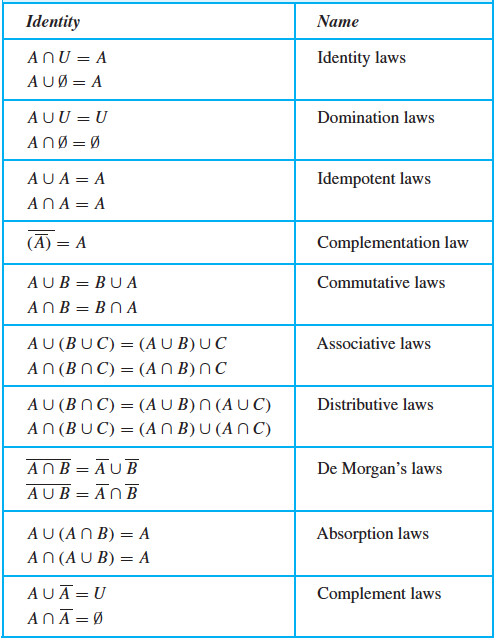
\includegraphics [scale=0.5]{Table-2-2-1-SetIdentities}
   \caption{Set Identities}
   \label{table:Set Identities}
\end{table}


\begin{notes}
Note the similarity to Identities of Logic 
\end{notes}

\section {Venn Diagrams}
    Diagrams that represent sets as ovals within a square box with or without labeled elements are called Venn diagrams. The outer box represents the universe of discourse, $U$, for the sets.   In a Venn diagram, the universal set is th einterior of a rectangle. If $A \subset B$, then the area of $A$ will be contained within the area of $B$.
If $A$ and $B$ are disjoint, then the area of $A$ will overlap art of the area of $B$.



\section {Set Cross Product}
    \subsection {Definition}
    \begin{definition}
The ordered n-tuple $(a_1, a_2, . . . , a_n)$ is the ordered collection that has $a_1$ as its first element, $a_2$ as its second element, . . . , and $a_n$ as its $n$th element.
Two tuples are considered equal if and only if all corresponding elements of the two tuples match.
    \end{definition}

    \begin{definition}
    Let $A$ and $B$ be sets. The Cartesian product of $A$ and $B$, denoted by $A \times B$, is the set of all
ordered pairs $(a, b)$, where $a \in A$ and $b \in B$. Hence,
$A \times B = \{(a, b) | a \in  A \land b \in B\}$.
    \end{definition}
$A \times B$
\begin{notes}
The elements of a tuple are ordered. $(a,b)$ is not the same as $(b, a)$.\\
Cross products of sets to themselves can be represented with superscripts. $A^2=A \times A$.\\
The cross product is a SET of TUPLES.
\end{notes}

    \begin {definition}
    The Cartesian product of the sets $A_1,A_2, . . . , A_n$, denoted by $A_1 \times A_2 \times \dots \times A_n$, is the
set of ordered n-tuples $(a_1, a_2, . . . , a_n)$, where $a_i$ belongs to $A_i$ for $i$ = 1, 2, . . . , n. In other
words,
$A_1 \times A_2 \times \dots \times A_n = \{(a_1, a_2, . . . , a_n) | a_i \in A_i$ for $i = 1, 2, . . . , n\}$.
    \end {definition}

\section {Set Cardinality}
\begin {definition}
The size of the set is the number of elements in the set for sets with a finite number of elements. We will defer infinite sets until later. This is called the set \textit{cardinality}. It is denoted by $\mathbf{card}(S)$ or $|S|$.
\end{definition}

\section {Powerset}
A special set called the power set is that set which includes every possible and unique subset of some set $S$. 
Note: the easiest way to enumerate the subset is by the number of elements in the set. List all the subsets with zero members (only one, the null set). Then all the subsets of size 1, 2, etc. 
\begin {theorem}
If the size of set $S$ is $m$, there are $2^m$ posible subsets.
\end{theorem}

Special symbol  $\mathcal{P} (A)$ designates the power set of set A.

\begin{notes}
the powerset IS A SET of SETS
\end{notes}


\section {Indexed Sets/Indexed Classes of Sets and Generalized Set Operations }
%NOTE: the requires functions!!
Let $I$ be any nonempty set (not necessarily a numeric set), and let $S$ be a collection of sets. An indexing function from $I$ to $S$ is a function $f:I \rightarrow S$. For an $i \in I$, we denote the image $f(i)$ by $A_i$. Thus we can say:

$\{A_i : i \in I\} or \{A_i\} \in I$, or simply $\{A_i\}$

The set $I$ is called the \textbf{indexing set} and the elements of $I$ the \textbf{indices}. 

When many sets are joined or intersected, we introduce an indexed notation:


$\cup _{ i=1} ^ n a _{i}$

$\cap_{ i=1} ^ n a _{i}$


(give Venn diagram)



\section {Fundamental Products of Sets}
Consider a set of sets $A_1$, $A_2$, etc that are all unique. 
Now let $A_i^*$ mean either $A_i$ or  $A_i^c$, that the notation $A_i^*$ either means $A_i$ or it means $A_i^c$.
The fundamental product of the set $S$ is that is the union of all sets denoted by $A^*$

\begin{notes}
there are m sets, $2^n$ such fundamental products (why?)
any two fundamental products are disjoint
the union of all the fundamental products is the universal
\end{notes}


\section {Partitions of a Set}
\begin{definition}
A \textbf{partition} of a set $S$ is a collection of disjoint nonempty subsets of $S$ that have $S$ as their union. Equivalently we can say the collection of subsets $A_i$, $i \in I$ where $I$ is an index set) forms a partition if and only if
$$A_i \neq \emptyset \text{  for  } i \in I$$
$$A_i \cup A_j =  \emptyset \text{  when  } i \neq j$$
$$\bigcup_{i \in I} A_i = S$$
\end{definition}

\section {Multisets and Bags}
A \textit{multiset} is a set that does not require each object to be unique. It can be represented by a set of pairs with the first element of the pair representing the object and the second representing the \textit{multiplicity} of that object in the multiset. These are sometimes called \textit{bags}

Sometimes the number of times that an element occurs in an unordered collection matters. Multisets are unordered collections of elements where an element can occur as a member more than once. The notation $\{m_1 \cdot a_1, m_2 \cdot a_2, \dots ,m_r \cdot a_r\}$ denotes the multiset with element $a_1$ occurring $m_1$ times, element $a_2$ occurring $m_2$ times, and so on. The numbers $m_i, i=1,2,3, \dots r$ are called the multiplicies of the elements $a_i, i=1,2,3, \dots ,r$.

%Sometimes the number of times that an element occurs in an unordered collection matters. Multisets are unordered collections of elements where an element can occur as a member more than once. The notation {m1 · a1, m2 · a2, . . . , mr · ar } denotes the multiset with element a1 occurring m1 times, element a2 occurring m2 times, and so on. The numbers mi , i = 1, 2, . . . , r are called the multiplicities of the elements ai , i = 1, 2, . . . , r.

\section{Strings}
We noted that a set cross product may not have a numeric sets but may map to some arbitrary set of symbols. The set of English letters can be the set. If we let the symbol $\Sigma$ represent a set of unique symbols then we can represent the set of all pairs as $\Sigma^2$, all triples as $\Sigma^3$, etc and we call $\Sigma$ an \textbf{alphabet}. We can extend this concept to a set of strings that do not all need to be the same length. Since members of $\Sigma$ are distinct and unique, there is no ambiguity in dropping the parentheses when representing the set of strings. 

Strings have some special notation and definitions. The string that contains no elements is the empty string, represented by a lower case lambda, $\lambda$. A string may be called a word.





    \subsection {Kleene Star notation}
Sometimes we wish to discuss all the possible strings that could be constructed  We can construct exactly one sequence of length zero from a alphabet $\Sigma$ which we represent as $\lambda$. If the domain of the sequence has $m$ elements, it is possible to construct $m$ strings (words) of length 1, $m^2$ of length 2, $m^3$ of length 3, etc. We will often want to talk about strings that can be of any length but only contain elements drawn from the codomain. This will be the union of the set of length zero, the sets of length 1,2,3, ... to infinity. This set of all possible strings drawn from the set is called the Kleene closure and designated $K_*$

We can talk about binary numbers as strings. 
$\mathbb{B}^2$ designates the set of binary strings of two bits.  \{00,01,10,11\}\\
$\mathbb{B}^8$ designates the set of 8 binary strings $\{00000000, 00000001, 00000010, \dots ,11111111\}$ \\
$\mathbb{B}^*$ represents the set of all possible binary strings.

\newpage






                     %%% FUNCTIONS %%%
\chapter {Functions}

\section {Definition}

\begin {definition}
Let $A$ and $B$ be non-empty sets. A function $f$ from $A$ to $B$ is an assignment of exactly one element in $B$ to each element in $A$. The set $A$ is called the domain of the function and the set $B$ is called the co-domain. The element from the domain, $a$ is called the pre-image and the element $b$ from the co-domain is called the target or image. The set of all images is called the range (note difference from co-domain).
\end {definition} 

\begin {definition}
If $f$ is a function from $A$ to $B$, we say that $A$ is the \textit{domain} of $f$ and $B$ is the \textit{codomain} of $f$. If $f(a)=b$, we say that $b$ is the \textit{image} of $a$ and $a$ is the \textit{preimage} of $b$. The \textit{range},or \textit{image}, of$f$ is the set of all images of elements of$A$. Also, if$f$ is a function from $A$ to $B$,we say that $f$ \textit{maps} $A$ to $B$. 
\end {definition}

\begin {definition}[function equality]
Two functions are \textbf{equal} when they have the same domain, have the same codomain, and map each element of their common domain to the same element in their common codomain.
\end {definition}
Note that if we change either the domain or codomain they are different functions.

Note that $f_1 + f_2)$ and $f_1 f_2$ are defined for real and integer valued functions.

\subsection {Set Builder Notation for Functions}

\subsection {Domain, Co-domain, Range, Pre-image, Image}

\subsection {Function signature, Function definition}
The signature of the function gives the function name, the domain and the co-domain and is written as:
$$f:A \rightarrow B$$ 
where $f$ is the function name, $A$ is the domain and $B$ is the co-domain and is read ``the function f from A to B''. \\
assigned\_grade: \{students\} $\rightarrow$ \{grades\}\\
The function definition gives the information needed to determine which element from the co-domain is the image of the element from the domain. This is called the function definition. 
$$f(a)=b$$

Sometimes called a mapping or transformation.

\subsection {Function Equality}

\subsection {Functions are subsets of set cross products, maplets}
All functions are subsets of the cross product of the domain and co-domain. A listing of all pairs is a valid function definition as is a table. Some authors will note specific mappings from an element a in the domain to the element b in the co-domain with the maplet notation:
$$ a \mapsto b$$ 



Sometimes we want to 

domain, co-domain, image, target, maplet, scope
function signature versus definition
graphic representation, arrow diagrams
well defined/proper function, partial functions
functional equality
graphic representation, analytic geometry (recognizing incomplete functions and non-functions)
Function versus operator

$f:S \rightarrow T$
The function f is a function that takes an argument from the set S and gives a result from the set T. S is the domain and T is the co-domain.

For function application we typically write $f(s)=t$ where $t$ is some expression based on $s$ and a method by which we can determine the unique element $t$ that $s$ maps to and can define the function using this notation. For example the function f might double the argument and add one which can be expressed as:

$f(x) = 2*x + 1$

When x is bound to a value, it results in a maplet from a member of the domain to some member in the codomain.

$f(2)=5$
or maplet $2 \mapsto 5$

For finite functions note that a function can be fully defined just by listing all the maplets of the function.

\subsection {Operators versus Functions}
We are used to the functional notation of algebra
$$  g(x,y)$$
We are also accustomed to operators from programming languages
$$x+y$$
If the function g is defined as the sum of the two arguments, the two notations mean the same thing. The second form is called operation notation and works well for both binary and unary operators. But for arguments of more than 2 it is difficult to use. Note that the usual form is infix. But if we adopt a different convention, putting the operator after all the arguments, it is now possible to have functions of any number of arguments written in operator notation with no loss of precision. If the operator follows the operands, the notation is called post-fix. If the operator preceeds the operands, it is called prefix. Thus the function notation, prefix, infix, and suffix notation for addition are
$$+(a,b)$$
$$ab+$$
$$a+b$$
$$+ab$$
Note that the C language has a way of converting a symbol into an infix operator for a binary function.

\subsection {Total and Partial Functions}
A total function is one that has a maplet for every element in the domain. These are called well defined functions. Some functions are undefined for some elements in the domain and these are called partial functions. Note that division on two numbers is a partial function. It is represented by an line through the arrow from domain to co-domain.

Not every element in the co-domain may be the image of an element in the domain. The set of all images is called the scope of the function.

\begin{definition}
A \textit{partial function} $f$ from a set $A$ to a set $B$ is an assignment to each element $a$ in a subset of $A$, called the \textit{domain of definition} of $f$ , of a unique element $b$ in $B$. The sets $A$ and $B$ are called the \textit{domain} and \textit{codomain} of $f$ , respectively. We say that $f$ is \textit{undefined} for elements in $A$ that are not in the domain of definition of $f$. When the domain of definition of $f$ equals $A$, we say that $f$ is a \textit{total function}. The notation $h:A \nrightarrow B$ is often used as a notation to designate a partial function $h$ that maps the set $A$ to $B$ where the set $A$ has undefined elements for the function $h$.
\end{definition}


\section {Properties of Functions}
    \subsection {Onto or Surjective Functions}
    \begin{definition}
    A function $f$ from $A$ to $B$ is called \textit{onto}, or a \textit{surjection}, if and only if for every element $b \in B$ there is an element $a \in A$ with $f(a)=b$. A function $f$ is called \textit{surjective} if it is onto.
    \end{definition}
    \begin{notes}
    A function $f$ is onto if $\forall y \exists x(f(x)=y)$, where the domain for $x$ is the domain of the function and the doman for $y$ is the codomain of the function.
    \end{notes}

    \subsection {One-to-One, Into, Injective}

    \subsection {One-to-One-Correspondence, One-to-One-Mapping, Bijective}

    \subsection {Inverse of a Function}
    \begin{definition}
    Let $f$ be a One-to-One-Correspondence from the set $A$ to the set $B$. The inverse function of
$f$ is the function that assigns to an element $b$ belonging to $B$ the unique element $a$ in $A$
such that $f (a) = b$. The inverse function of $f$ is denoted by $f^{-1}$. Hence, $f^{-1} (b) = a$ when
$f (a) = b$.
    \end{definition}


\section {Composition of Functions}

\section {Common functions in computer science}
    \subsection {Functions of Real to Integer}
floor, ceiling, integer
    \subsection{Functions of Boolean to Integer}
Boolean $\leftrightarrow$ Integer

    \subsection {Functions of Boolean to Real}
Boolean $\leftrightarrow \mathbb{R}$ 

    \subsection {Other Functions}
polynomial, log, log-linear, exponential
increasing/decreasing versus strictly increasing and decreasing
cipher function
permutation function



\section {Composition of Functions}

Properties of Functions: Onto, One-to-One, One-to-One Correspondence, Invertible
An invertible function is called a permutation

Elementary Functions Used in Computer Science and Engineering
exponential and logarithmic, floor and ceiling, integer and absolute value, remainder function (MOD operator in programming), integer to binary and binary to integer, from natural numbers to integers.


\section {Graphic Representations of Functions: Set mappings and analytic geometry}
    \subsection {Representing Functions as Graphs}
        \subsubsection {Introduction to Graphs}
vertices or nodes, edges (directed or undirected), head, tail, in-degree, out-degree, self-loop (reflexive), 

    \subsection {Representing Functions with Analytic Geometry}
Note how properties of a graph can be read from the plots.

\section {Sequences}
Formally, a sequence can be defined as a function whose domain is either the set of the natural numbers (for infinite sequences) or the set of the first n natural numbers (for a sequence of finite length n). The position of an element in a sequence is its rank or index; it is the natural number from which the element is the image. It depends on the context or a specific convention, if the first element has index 0 or 1. When a symbol has been chosen for denoting a sequence, the nth element of the sequence is denoted by this symbol with n as subscript; for example, the nth element of the Fibonacci sequence is generally denoted Fn.

In mathematics a \textit{finite sequence} is usually defined as any function $f$ whose domain is a finite initial set $\{1,2,3, \dots ,n\}$ of positive integers. The number $n$ of integers in the domain of $f$ is the \textit{length} of $f$. When considering $f$ as a finite sequence it is customery to write
$$f_1,f_2, \dots$$
rather than
$$f(1),f(2), \dots$$
in designating the value of $f$ at 1,2, \dots.

Along with this subscript notation there is the \textit{n-tuple} notation
$$(f_1,f_2, \dots f_n)$$


$f_i$ is the $i_{th}$ \textit{entry} or \textit{term} of $f$. This \textit{n-tuple} notation indicates how explicit short finite sequences can be defined and pictured. For example, the equation  
$$x=(5,1,4,0)$$
tells us that $x$ is the finite sequence of length 4 whose values on its domain \{1,2,3,4\} are given by
$$x_1=x(1)=5$$
$$x_2=x(2)=1$$
$$x_3=x(3)=4$$
$$x_4=x(4)=0$$

The most common domain for a sequence is $\mathbb{N}$. However it is frequently more convenient to use natural numbers including zero. There is an edge case where sometimes the domain is the null set in which case the sequence is empty and can be shown using a pair of empty parentheses to emphasize that there are no terms in the sequence
$$(  )$$

Consider a function $\sigma:\mathbb{N} \rightarrow \mathbb{Z}$
For example sigma(x)=2*x
this gives maplets 1|->2, 2|->4, etc
Since the domain is understood to be natural numbers it is easier to just write the images as a list:
2,4,6,8, etc
We can use subscript notation and state this more abstractly:

A sequence A is a(1),a(2),a(3),...a(i) 
or
$\{a(n) n \in N\}$  or even more compactly as \{a(n)\} when it is understood we intend a sequence. It is common in sequences to base not strictly on natural numbers but natural numbers plus the member zero. 

Note that this definition of sequence allows for non-numeric sequences.









Evaluation of Functions
Some functions are trivially evaluated.

f(x)=2*x

Others will have values that must be calculated

f(x)=sin(x)

The way a value is assigned to a function by calculation is the starting point for computer science and leads to a discussion of algorithms we will take up later.


\section {Growth of Functions and Asymptotic Notation}\
You know that some functions "grow" faster than others. For example you know that a quadratic polynomial will overtake a linear polynomial. But many linear functions will evaluate to higher numbers for small values. We want some way to express the concept that a quadratic is in some sense bigger. This leads to a new notation, the Big-O or asymptotic notation.

While it may be true that some functions on n may evaluate to larger numbers for smaller values, there will be a point at which the "bigger" function will overtake and forever remain larger. Let us call this point n sub zero. If we can find some n sub zero such that all higher values of n will remain larger, we have demonstrated that the function is in this sense "larger".

Given two linear polynomial equations, we can always do this by changing the values of the constants. But no matter how you change the constants of a linear polynomial, a quadratic polynomial will always overtake it. This shows that a quadratic will ALWAYS beat a linear function, that they are in some sense in different categories regardless of the choice of constants. This gives us the concept of the category of the function or the order or magnitude designated by Big O. We can change any linear function into another linear polynomial function by changing the constants. We group all of these together and call them linear polynomial functions or polynomial functions on n, written O(n). We can prove that there are at least 7 categories that are important to the study of computer science, constant O(1), linear O(n), log O(log n), log-linear O(n log n), quadratic O(n**2), exponential O(2**n), and factorial O(n!). Note that each of these is a grouping of functions that include all the variations of different constants. By choosing the constants, we can always find some n sub 0 such that a quadratic will beat a linear. This gives us an ordering of these categories

O(1) < O(log n) < O(n) < O(n log n) < O(n**2) < O(2**n) < O(n!)

For any two specific functions of different categories one can find the n sub 0 at which the larger function overtakes the smaller and forever remains ahead. This way of viewing the relative size of functions will be used when we study the complexity of algorithms later.




\section {Sigma Notation, Summations and Open Form Formulas}
One common function performed on numeric sequences is summation. For this we use the capital sigma. $\Sigma_{j=1}^{n} a_j = a_1 + a_2+ ... + a_n$

It may start at something other than 1 and may sum to infinity. The letter j is called the dummy index or dummy variable.

\section {Recursively defined functions}
Open form solution

\section {Functions on Functions; first class objects}

\newpage









                      %%% RELATIONS %%%
\chapter {Relations}

Relations are closely associated with functions but we looked at those first since you are familiar with them from before. Relations are a superset of functions, all functions are relations but not all relations are functions.

The fundamental restriction to a function is that it needed to evaluate to exactly one value. A relation can be a many-to-many mapping from the domain to the codomain. In its most abstract statement, all valid subsets of the cross product of the domain and codomain are relations.

A fundamental paragigm is one called objects/relations and is found in programming languages today. We saw that sets are collections of objects and we saw that predicates take on the value true when a particular property is found in that object. Objects can have relationships among them and the most basic is the binary relationship. In a binary relationship we way that the two objects either are in or not in that relationship with each other. This chapter explores the consequences of this and its many applications.



\section {Binary Relations}
\begin {definition}
Let $A$ and $B$ be sets. A \textit {binary relation between $A$ and $B$} is a subset of $A \times B$.
\end {definition} 

A relation among any number of sets is a subset of their cross product. 
aRb, a is related to b
     , a is not related to be
In a binary relation, the domain is the domain of the relation is the set of all first elements of the tuples. The range is the set of all second members of the pairs. 

    \subsection {Functions as Relations}

\section {Relations on a Set}
\begin {definition}
A \textit{relation on the set A} is a relation from $A$ to $A$
\end {definition}

    \subsection {Relational operators}
    


\section {Properties of Relations: reflexive, symmetric, anti-symmetric, transitive, Closure}
    \subsection {Reflexive Relations}
    \begin {definition}
    A relation $R$ on a set $A$ is called \textit{reflexive} if $(a,a) \in R$ for every element $a \in A$. The relation $R$ is reflexive if $\forall a((a,a) \in R)$.
    \end {definition}
    
    \subsection {Symmetric Relations}
    \begin {definition}
    A relation $R$ on a set $A$ is alled \textit{symmetric} if $(b,a) \in R$ for all $a,b \in A$.
    \end {definition} 
    
    \subsection {Anti-Symmetric Relations}
    \begin {definition}
    A relation $R$ on set $A$ such that for all $a,b \in A$, if $(a,b) \in R$ and $(b,a) \in R$, then $a=b$ is called \textit{antisymmetric}
    \end {definition}
    
    \subsection {Transitive Relations}
    \begin {definition}
    A relation $R$ on a set $A$ is called \textit{transitive} if whenever $(a,b)\in R$ and $(b,c) \in R$, then $(a,c) \in R$. The relation $R$ on a set $A$ is transitive if we have $\forall a \forall b \forall c (((a,b) \in R \land (b,c) \in R) \rightarrow (a,c) \in R)$
    \end {definition}
    
    \subsection {Anti-Reflexive}


\section{Representations of Relations}

\section{Closures on Relations}
  \subsection{Closures}
  \subsection{Paths in Directed Graphs}
  \subsection{Transitive Closures}
  \subsection{Computing Transitive Closures} Warshall's Algorithm


\section {Equivalence Relations}
reflective, symmetric, transitive
remainder function partitions

    \subsection {Equivalence Classes and Set Partitions}

\begin{definition}
The elements $a$ and $b$ that are related by an equivalence relatin are called \textit{equivalent}. The notation $a \sim b$ is often used to denote that $a$ and $b$ are equivalent elements with respect to a particular equivalence relation.
\end{definition}

\begin{definition}
Let $R$ be an equivalence relation on a set $A$. The set of all elements that are related to an element $a$ of $A$ is called the \textit{equivalence class} of $a$. The equivalence class of $a$ with respect to $R$ is denoted by $[a]_R$. When only one relation is under consideration, we can delete the subscript $R$ and write $[a]$ for this equivalence class.

If $b \in [a]_R$, then $b$ is called a \textbf{representative} of this equivalence class.
\end{definition}


\begin{theorem}
Let $R$ be an equivalence relation on a set $A$. These statements for elements $a$ and $b$ of $A$ are equivalent:
\begin{enumerate}[label=(\roman*)]
\item
$aRb$
\item
$[a]=[b]$
\item
$[a] \cap [b] \neq \emptyset$
\end{enumerate}
\end{theorem}

\begin{theorem}
Let $R$ be an equivalence relation on a set $S$. Then the equivalence classes of $R$ form a partition of $S$. Conversely, given a partition $\{A_i | i \in I\}$ of the set $S$, there is an equivalence relation $R$ that has the sets $A_i, i \in I$, as its equivalnece classes.
\end{theorem}

    \subsection {Partial Ordering Relations}
reflexive, antisymmetric, transitive
Given a set Sand an ordering relation R on S,  the pair (S, R) is called a partially ordered set or poset. Note code.

    \subsection {Posets}
    \subsection {Comparability}
    \subsection {Comparability, Linearly Ordered Sets}
Note that not all pairs in the set S need be in relation. If for two elements of the set S, a, b aRb then we say a and b are comparable under R. If not, they are incomparable written a||b

Suppose all elements in the set are pairwise comparable. Such a poset is then called a totally ordered or linearly ordered set and S is called a chain. 

    \subsection {Lexicographic Order}
    \subsection {Haase Diagrams and Posets}
    \subsection {Maximal and Minimal Elements}
    \subsection {Topological Sorting}
    
\section {Inverse relation}
An operation on a relation is to take the inverse.

\section {Composition of Relations}


\section {Graphic Representation of Relations}
For relations onto themselves, this gives what we will later call a directed graph. We cover graphs more formally in a later chapter.
    \subsection {Graphs and Digraphs}

\section {Closure Property of Relations}
   \subsection {Transitive Closure of Relations}
   \subsection {Kleene Closure and Order}

\section {N-ary Relations}
    \subsection {Application to Databases}

\section {Matrices and Linear Algebra}
Many include matrices in Discrete Mathematics. We exclude this since it is offered as a separate course.
\newpage


                       %%% ALGORITHMS %%%
\chapter {Algorithms}
Relative to many texts on discrete math, this chapter is sparse because most of the material overlaps with a standard undergraduate course that will focus on algorithms and their analysis. The emphasis for these notes is simply the mathematical concept and its relationship to the structures needed to approach computation from a theoretical perspective.

\begin{definition}[Definition of Algorithm from Rosen]
An \textit{algorithm} is a finite set of precise instructions for performing a computation or for solving a problem.
\end{definition}
\begin{definition}[Definition of Algorithm from Schaums]
An algorithm $M$ is a finite step-by-step list of well-defined instructions for solving a particular problem, for instance to evaluate a function $f$ given an argument $X$ where $X$ may be any mathematical structure. Frequently there may be more than one algorithm to computer $f(X)$ and we need tools to analyze the differences between the different algorithms.
\end{definition}

\begin{notes}
A pre-requisite to this class is at least one programming course so the student is expected to understand the conventions of a procedural language used to describe an algorithm. There is no universal way to describe an algorithm since programming languages will often use different ways of doing the same thing. The conventions of this book come from Rosen which represents a common notation that uses conventions from mathematics as well as programming languages.
\end{notes}

\section{Searching Algorithms}
\section{Sorting Algorithms}

\section{The Halting Problem}
\begin{theorem}
There is no algorithm that accepts an algorithm and some input data set as input and determines whether it will halt.
\end{theorem}

Every function has a method by which a value can be calculated. This often comes from calculus for many of the functions used in engineering but not always. For example we have a way of calculating the factorial function that uses only basic arithmetic. Regardless of how it is calculated you will note that they all have very specific steps that must be executed in some order that are well defined. This is called an algorithm. Computer science began with the proof that any well defined algorithm could be mechanically executed by a machine instead of a human. The term computer originally meant a human using computation tools like an adding machine to execute the steps needed to determine the values. These values of the functions were published in books and the function was evaluated by a lookup in a table instead of on-the-spot calculation.

Not all functions take in single parameters. Some, like the permutation function, will take in a large number of values and produce some permutation of those numbers. Sorting is just such a function. Clearly the work done by the sorting function will depend on the size of the input set which we call n. 

For practical reasons, we are interested in how long an algorithm will take given a particular set of numbers as input. This becomes a different function T for this algorithm which has as input the size of the input set, n. The time a specific algorithm will work on a particular input set before giving a result is the functionT(n). You might naively assume that T(n) will always result in the same value for any size input but you would be wrong. The T function will vary with both the size but also the specific input. For example some sort algorithms will have T(n) in the category of O(n) for sorted input but O(n**2) for out of order input. The big O of the algorithm will vary with the algorithm and its input.

While we are sometimes interested in the best-case scenario for the algorithm and its input set, we most often are more interested in the worst case scenario. What will be the big O for this algorithm over all the possible inputs it could get? This defines an upper bound for the complexity of this algorithm. Since the worst and best case for an algorithm may have functions from different categories, the best case may be in a different big O category. When analyzing algorithms, we call this the lower bound for that function on T(n). We give this the name Omega. When we find one category that contains both the upper and lower bound, we call this the Theta of that function. When we find a Theta for an algorithm we say we have found the tight upper bound 

We defer the further study of algorithmic complexity to your course on Algorithms in your undergrad program.


\section {Analysis of Algorithms}
  \subsection{The Time Function of an Algorithm}
  We want to analyze how long an algorithm takes, called the time complexity of the algorithm. First note that many algorithms will use different numbers of steps depending upon the input they are given. So this is not a fixed function from algorithm to time but instead a range of values. The time might be computable for specific algorithm and a specific input but in general what we want is the range of possible times for this algorithm. Of all the possible ways we can analyze the performance of an algorithm the most basic is to look at the relationship between the ``size'' of the input and the time ignoring all other considerations. We represent this ``size'' as $N$. We call the time function $T$ so we want to perform asymptotic analysis on the function $T(N)$.

Given this range, we might be interested in the best possible time, the worst possible time and/or the average time this algorithm will use over some set of input values. The most frequently analyzed is the worst case time and we present how that is described. We will use asymptotic function analysis (chapter on functions) to do this. 

While it is true that the time required to execute an instruction varies with the machine and even within a machine the instruction to be executed. For example a divide instruction is longer than a move. But this relationship is fixed, for the most part, and can be ignored for the purposes of asymptotic analysis. 

The most common analysis is relative to the economic reality of time. But a comparable analysis can be done for space requirements too. In fact any resource needed to run the algorithm can be subjected to analysis in a comparable way.

We stop our discussion of algorithmic analysis here and leave it to a course devoted to this subject.
\newpage




                       %%%   INTEGERS   %%%
\chapter {Integers}
A math major will be expected to complete a course in Number Theory but few computer science programs require it. Yet there are a few concepts from number theory that are important for a computer science student to understand to be prepared for either a career in software engineering or the pursuit of graduate school in computer science. This chapter seeks to limit the material to those two objectives only.
\textbf{number theory}
\section{Division}
\begin{definition}
If $a$ and $b$ are integers with $a \neq 0$, we say that \textit{a divides b} if there is an integer $c$ such that $b=ac$. When $a$ divides $b$ we say that $a$ is a \textit{factor} of $b$ and that $b$ is a \textit{multiple} of $a$. The notation $a \vert b$ denotes that $a$ divides $b$. We write $a \not\vert b$ when $a$ does not divide $b$.

When the domain of discourse is the set of integers, we can express $a\vert b$ as $\exists c(ac=b)$.
\end{definition}



\begin{theorem}
Let $a$, $b$, and $c$ be integers. Then 
\begin{enumerate}
\item if $a \vert b$ and $a \vert c$, then $a \vert (b+c)$;
\item if $a \vert b$, then $a \vert bc$ for all integers $c$;
\item if $a \vert b$ and $b \vert c$, then $a \vert c$.
\end{enumerate}
\end{theorem}

\begin{corollary}
If $a$, $b$, and $c$ are integers such that $a \vert b$ and $a \vert c$, then $a \vert mb+nc$ whenever $m$ and $n$ are integers.
\end{corollary}


\section {The Division Algorithm}
\begin {theorem} [The Division ``Algorithm'']  Let $a$ be an integer and $d$ a positive integer. Then there are unique integers $q$ and $r$, with $0 \leq r < d$, such that $a=dq+r$.
\end {theorem}


\begin {definition}
In the equality given in the divison algorithm $d$ is called the \textit{divisor}, $a$ is called the \textit{dividend}, $q$ is called the \textit{quotient} and $r$ is called the \textit{remainder}. This notation is used to express the quotient and remainder:
     $$ q=a\; \mathbf{div} \;d, \;\;   r=a\; \mathbf{\bmod}\; d. $$
\end {definition}

\begin{notes}
The binary operator \textbf{div} in this definition is the same as a programming integer divide. 
This definition of $\bmod$ defines a function since $r$ is uniquely determined.\\ 
Note how this is calculated for negative integers.\\
Note how some programming languages had not always calculated this properly.
\end{notes}

\section {Modular Arithmetic}
In some applications, we only care about the remainder. Consider time or degrees. We have special notation for this concept.

\begin{definition}
If $a$ and $b$ are integers and $m$ is a positive integers, then $a$ is \textit{congruent to b modulo m} if $m$ divides $a-b$. We use the notation $a \equiv b$ (modulo $m$) or $a \equiv b (mod m)$
\end {definition}

\begin{notes}
Be careful not to confuse \textbf{mod}, a function with (mod $m$). The first is a binary function used as an infix operator while the second is a qualification for the entire equivalence. Authors use different notations to mean one or the other. The (modulo $m$) equivalence is NOT a function since one integer can be in equivalence to multiple integers, modulo $m$.
\end{notes}

\begin{theorem}
Let $a$ and $b$ be integers, and let $m$ be a positive integer. Then $a   \equiv b$ (mod $m$) if and only if $a   \mathbf{mod} m = b   \mathbf{mod} m$ 
\end{theorem}

\begin{theorem}
Let $m$ be a positive integer. The integers $a$ and $b$ are congruent modulo $m$ if and onl if there is an integer $k$ such that $a=b+km$.
\end{theorem}


\begin{theorem}
Let $m$ be a positive integer. If $a \equiv b$ (mod $m$) and $c \equiv d$ (mod $m$), then $a+c \equiv b+d$ (mod $m$) and $ac \equiv bd$ (mod m).
\end{theorem}

\begin{definition}
The set of all integers congruent to an integer $a$ modulo $m$ is called the \textbf{congruence class} of $a$ modulo $b$ or the \textbf{congruence classes modulo $m$}.
\end{definition}

\begin{corollary}
Let $m$ be a positive integer and let $a$ and $b$ be integers. Then
$$(a+b) (\mod {m}) = ((a \mod {m}) + (b \mod  {m} )) \mod {m}$$
and
$$ab \mod{m} \equiv ((a \mod{m})(b \mod{m}) \mod{m}$$
\end{corollary}



  \subsection {Applications of Congruences}
Hashing Functions
Pseudorandom Numbers
Check Digits

  \subsection {Cryptology}

\section {Primes and Greatest Common Divisors}
  \subsection {Primes}
\begin{definition}
A positive integer $p$ greater than 1 is called \textit{prime} if the only positive factors of $p$ are 1 and $p$. A positive integer than is greater than 1 and is not prime is called \textit{composite}.
\end{definition}

\begin{notes}
The integer $n$ is composite if and only if there exists an integer $a$ such that $a \vert n$ and $1<a<n$.
\end{notes}

\begin{theorem} [The Fundamental Theorem of Arithmetic]
Every positive integer greater than 1 can be written uniquely as a prime or as the product of two or more primes where the prime factors are written in order of nondecreasing size.
\end{theorem}

\begin{theorem}
If $n$ is a composite integer, then $n$ has a prime divisor less than or equal to $\sqrt{n}$
\end{theorem}

\begin{theorem}[The Infinitude of Primes]
There are infinitely many primes.
\end{theorem}

\begin{definition}
The number of primes not exceeding some real number $x$ is defined as the function $\pi(x)$.
\end{definition}

\begin{theorem}[The Prime Number Theorem]
The ratio of $\pi(x)$, the number of primes not exceeding $x$, and the expression $\frac{x}{\ln{x}}$ approaches 1 as $x$ grows without bound.\\
$\frac{\pi(x)}{x / ln x}$
\end{theorem}

  \subsection {Greatest Common Divisors and Least Common Multiples}
\begin{definition}
Let $a$ and $b$ be integers, not both zero. The largest integer $d$ such that $d \vert a$ and $d \vert b$ is called the \textit{greatest common divisor} of $a$ and $b$. The greatest common divisor of $a$ and $b$ is denoted by gcd(a,b).
\end{definition}

\begin{definition}
The integers $a$ and $b$ are \textit{relatively prime} if their greatest common divisor is 1.
\end{definition}

\begin{definition}
the integers $a_1,a_2, \dots a_n$ are \textit{pairwise relatively prime} if gcd($a_i,a_j$)=a whenever $1\le i < j \le n$.
\end{definition}

\begin{definition}
The \textit{least common multiple} of the positive integers $a$ and $b$ is the smallest positive integer that is divisible by b oth $a$ and $b$. The least common multiple of $a$ and $b$ is denoted by lcm($a$,$b$).
\end{definition}

\begin{definition}
The value of the \textbf{Euler $\phi$-function} at the positive integer $n$ is defined to be the number of positive integers less than or equal to $n$ that are relatively prime to $n$. 
\end{definition}







\section {Integers and Algorithms}
  \subsection {Representation of Integers}
\begin{theorem}[Base b Expansion of n]
Let $b$ be a positive integer greater than 1. Then if $n$ is a positive integer, it can be expressed uniquely in the form
$$n=a_kb^k+a_{k-1}b^{k-1}+ \dots +a_1b + a_0,$$
where $k$ is a nonnegative integer, $a_0,a_1, \dots,a_k$ are nonnegative integers less than $b$, and $a_k\neq0$. Choosing $b=1$ gives the conventional decimal expansion and choosing $b=2$ gives the binary expansion. Choosing $b=16$ gives the hexadecimal expansion. Choosing $b=8$ give the octal expansion.
\end{theorem}

\begin{notes}
Each hexadecimal digit is represented by four binary digits. Each octal digit is represented by three binary digits.
\end{notes}

Algorithm for the construction of a base b expansion.
  \subsection {Algorithms for Integer Operations}
Algorithm for the addition of integers.
Algorithm for the multiplication of integers.
Algorithm for the computation of div and mod.
  \subsection {Modular Exponentiation}
Algorithm for modular exponentiation.
You will find that in cryptography it is important to be able to find $b^n \mathbf{mod} m$ efficiently...
  \subsection {The Euclidean Algorithm}
\begin{lemma}
Let $a=bq+r$, where $a$,$b$,$q$, and $r$ are integers. Then gcd($a$,$b$)=gcd($b$,$r$)
\end{lemma}
Algorithm, The Euclidean Algorithm

\section {Applications of Number Theory}
  \subsection {Some Useful Results}
\begin {theorem}
If $a$ and $b$ are positive integers, then there exist integers $s$ and $t$ such that gcd($a$,$b$)=$sa+tb$
\end {theorem}
Algorithm, the extended Euclidean algorithm to find linear combinations.

\begin{lemma}
If $a$,$b$, and $c$ are positive integers such that gcd($a$,$b$)=a and $a \vert bc$, then $a \vert c$.
\end{lemma}

\begin{lemma}
If $p$ is a prime and $p \vert a_1a_2\dots a_n$ where each $a_i$ is an integers, then $p\vert a_1$ for some $i$.
\end{lemma}

\begin{theorem}
Let $m$ be a positive integer and let $a$,$b$ and $c$ be integers. If $ac\equiv bc(\mod m$) and gcd($c$,$m$)=1, then $a\equiv b(\mod m$)
\end{theorem}
  \subsection {Linear Congruences}



  \subsection {The Chinese Remainder Theorem}


  \subsection {Computer Arithmetic with Large Integers}

  \subsection {Pseudoprimes}

  \subsection {Public Key Cryptography}
  \subsection {The RSA Cryptosystem}
  
  \subsection {RSA as a Public Key System}








\section {Schaums material}
Associative
Commutative
Distributive
Additive and multiplicative identity
Additive inverse

\subsection {Order, Inequality, Absolute Value}
\subsection {Well Ordering Principle}
\subsection {Integers and Division}
\subsection {Primes}
\subsection {LCM}
\subsection {Fundamental Theorem of Arithmetic}
\subsection {Congruence Relation}
\subsection {Residue Classes}
\subsection {Congruence Arithmetic}
\subsection {Arithmetic of Residue Classes}
\subsection {Integers Modulo m, Zsubm}
\subsection {Cancellation Laws for Congruence}
\subsection {Reduced Residue Systems, Euler Phi Function}
\subsection {Congruence Equations}
    \subsection {Linear Congruence Equation}






\newpage



                                                                   %%%  INDUCTION AND RECURSION   %%%
\chapter {Induction and Recursion}
recursive definitions of sets

Recursion occurs throughout the study of computer science and this chapter must give you the basis to be able to understand the many ways in which it serves our discipline. The first is the concept of proving properties of infinite sets using a recursive argument. All recursive arguments have two parts that have the ladder as a metaphor. Ladders have rungs that are equally spaced. And one you are on a rung, if you can step up to the next one you know you can climb the ladder regardless how tall it may be. But the other vital part of the argument is that you can get onto the ladder in the first place. From this start we can explore the recursive definition of sets, recursive functions and relations and recursive algorithms. 
proving a truth for an infinite set


Note: Induction versus Deduction
Induction has two meanings. In common language induction is a way of generalizing over many observations. But in mathematics we use the word to describe a particular type of deductive reasoning that can prove that some properties of infinite sets must be true. We call this inductive reasoning. 



\section {Mathematical Induction}
\begin{notes}
Do not confuse mathematical induction with inductive reasoning. In logic deductive reasoning uses rules of inference to draw conclusions from premises, whereas inductive reasong makes conclusions only supported, but not ensured, by evidence. Mathematical proofs, incuding arguments that use mathematical induction, are deductive, not inductive.
\end{notes}

\begin{definition}[Principle of Mathematical Induction]
To prove that $P(n)$ is true for all positive integers $n$< where $P(n)$ is a propositional function, we complete two steps: \\
BASIS STEP: Verify that $P(1)$ is true.\\
INDUCTIVE STEP: Show that the conditional statement $P(k) \rightarrow P(k+1)$ is true for all positive integers $k$.
\end{definition}
 
    inductive hypothesis, ASSUME $P(k)$ is true. This is not the same as asserting it is true for all $k$ only that if the assumption holds that $P(k+1)$ must be true.
Expressed as a rule of inference it looks like this:
$$[P(1) \land \forall k (P(k) \rightarrow P(k+1))] \rightarrow \forall n P(n),$$














  \subsection {Mathematical Induction}
If a set is finite and we want to show some property holds for all elements, an iteration of testing for that property is always possible. But what if the set we examine is infinite? Many properties in mathematics are on infinite sets such as the set of integers or reals. Common examples are proving that for every positive integer $n$, $n! \leq n^n$. In general we are given some predicate $P$ (in this example that $n! \leq n^n$ and then asked to prove that this is a univeral property
$$\forall P(n), n\in \mathbb{N} \cup {0} | n! \leq n^n$$
For this and many other proofs of this kind we depend upon the Principle of Mathematical Induction. First prove that the proposition is true for the first element of the set. Then prove that if the propertly holds for some arbitrary element, $k$, that it must hold for the subsequent element, $k+1$. The principle gives you a new rule of inference that allows you to assert that the property must hold for every element of the set. More formally we state the principle of mathematical induction like this:\\
Basis Step: Prove $P(1)$ \\
Inductive Step: $P(k) \rightarrow P(k+1)$\\
Rule of Inference: $[P(1) \land \forall P(k) \rightarrow P{k+1}] \rightarrow \forall n P(n)$\\

We will call this the weak form of mathematical induction.

Note: The proofs always use a different variable name in the proof from the principle to be proved. In the example we were asked to prove for all n. But the proof worked with variable k. This is to emphasize that we may not assume that $P(k)$ is true. But we can still use it in a conditional expression that if $P(k)$ is true and we show that the implication that $P(k+1)$ must also be true, it does not matter if the antecedent of the conditional statement is false since we only need to show that in all cases where it is true that the consequent must also be true. Ignoring this subtle point of logic causes many people to commit the fallacy of affirming the consequent, or begging the question.


\section {Strong Induction and Well-Ordering}
Sometimes it is not sufficient to show that the universal is valid for $n=1$ to establish a base case. Sometimes there are two or more initial conditions that must be proven. This gives us a new form of mathematical induction call the strong form:\\
\begin{definition}[Strong Induction]
To prove that $P(n)$ is true for all positiv eintegers $n$, where $P(n)$ is a propositional function, we complete two steps: \\
BASIS STEP: We verify that the proposition $P(1)$ is true.\\
INDUCTIVE STEP: We show that the conditional statement $[P(1) \land P(2) \land \dots P(k)] \rightarrow P(k+1)$ is true for all positive integers $k$.
\end{definition}

\begin{definition}[Well-Ordering Property]
Every nonempty set of nonnegative integers has a least element.
\end{definition}
 

\section {Recursive Definitions and Structural Induction}
 
  \subsection {Recursively Defined Functions}
We can define functions using a recursive definition. Such definitions are called recursive or inductive definitions. Such functions are well defined since the value of the function at every integer is uniquely defined in a nonambiguous way.
\begin{definition}[Recurseively Defined Function]
We can define a function with the set of nonnegative integers as its domain with two steps:\\
BASIS STEP: Specify the value of the function at zero (the base case)\\
RECURSIVE STEP: Give a rule for finding its value at an integer from from its values at smaller integers.
\end{definition}

\begin{definition}
The \textit{Fibonacci numbers} $f_0,f_1,f_2, \dots$ , are defined by the equaltions
 $f_0=0$,\\
$f_1=1$, and \\
$f_n=f_{n-1} + f_{n-2}$ for all $n \ge 2$.
\end{definition}








  \subsection {Recursively Defined Sets and Structures}
basis step, recursive step, exclusion rule
An important use of recurseive definitions for sets is to define \textbf{well-formed formulae} of various types.

\begin{definition} \label{WFF} [Well-Formed Formulae of Compound Propositions]  Well-Formed formulae of a simple propositional statements can be defined as follows:\\
BASIS STEP: T, F, and $s$, where $s$ is a propositional variable, are well-formed formulae.\\
RECURSIVE STEP: If $E$ and $F$ are well-formed formulae, then $(\neg E)$, $(E \land F)$, $(E \lor F)$, $(E \rightarrow F)$, and $(E \leftrightarrow F)$ are well-formed formulae.
\end{definition}

\begin{definition}[$\Sigma^*$]
The set if all posible strings over the alphabet $\Sigma$ can be defined recursively by:\\
BASIS STEP: $\lambda \in \Sigma^*$ where $\lambda$
 is the empty string containing no symbols).\\
RECURSIVE STEP: If $w \in \Sigma^*$ and $x \in \Sigma$, then the concatenation $wx \in \Sigma^*$.
\end{definition}

A structure cal also be defined using a recursive definition.

\begin{definition}[The Set of Rooted Trees]
The set of rooted trees, where a rooted tree consists of a set of vertices containing a distinguished vertex called the root, and edges connectinve these vertices, can be defined recursively by these steps:\\
BASIS STEP: A single vertex $r$ is a rooted tree. \\
RECURSIVE STEP: Suppose that $T_1,T_2, \dots T_n$ are disjoint rooted trees with roots $r_1,r_2, \dots r_n$, respectively. Then the graph formed by starting with a root $r$, which is not in any of the rooted trees $T_1,T_2, \dots,T_n$, and adding an edge from $r$ to each of the vertices $r_1,r_2, \dots r_n$, is also a rooted tree.
\end{definition}

  \subsection {Structural Induction}
We can prove results about recursively defined sets using a form of mathematical induction. We do this by using a connection between recursively defined sets and mathematical induction.

\begin{theorem}
Let $S$ be a set recursively defined by:\\
BASIS STEP: $3 \in S$ \\
RECURSIVE STEP: If $x \in S$ and $y\in S$, then $x+y \in S$,
then all elements of the set $S$ are multiples of 3.
\end{theorem}

\begin{definition} [Proof by Structural Induction]
A proof by structural induction consists of two parts. These parts are:
BASIS STEP: Show that the result holds for all elements specified in the basis steop of the recursive definition to be in the set. \\
RECURSIVE STEP: Show that if the statement is true for each of the elements used to construct new elements in the recursive step of the definition, the result holds for these new elements.
\end{definition}
 
\begin{theorem}
Show that the set of well-formed formulae in \ref{WFF} will always have an equal number of left and right parentheses using structural recursion.
\end{theorem}



\begin{definition}
We define the height $h(T)$ of a full binary tree $T$ recursively.\\
BASIS STEP: The height of the full binary tree $T$ consisting of only a root $r$ is $h(T)=0$.
RECURSIVE STEP:  If $T_1$ and $T_2$ are full binary trees, then the full binary tree $T=T_1 \cdot T_2$ has height $h(T)=1 + max(h(T), h(T_2))$.
\end{definition}

\begin{theorem}
If $T$ is a full binary tree and$ n(T$) defines the number of nodes in a full binary tree $T$, then $n(T) \le 2^{h(T)+1} -1$
\end{theorem}

  \subsection {Generalized Induction}
\begin{definition}
The \textbf{reversal} of a string $w$ is the string consisting of the symbols of the string in reverse order. The reversal of the string $w$ is denoted $w^R$.
\end{definition}

Ackermann's (ex 47)

\section {Recursive Algorithms}
  \begin {definition}
An algorithm is called \textit{recursive} of iot solves a problem by reducing it to an instance of the same problem with smaller input.
\end{definition}

  \subsection {Proving Recursive Algorithms Correct}
  \subsection {Recursion and Iteration}
A recursive algorithm will compute a value by taking the function evaluation at the requested value and recursively computing smaller values. The function can also be computed by taking the value at the base case and applying the recursive rule until the requested value is determined, changing a recursive algorithm into an interative algorithm.

  \subsection {The Merge Sort}

\

\newpage


                                                                              %%%  COUNTING  %%%%%%%%%%%%%%%
\chapter {Counting}
We need to count the operations of an algorithm to comput its time complexity.

\section {The Basics of Counting}
    \subsection {Basic Counting Principles}
product rule, sum rule.
To count means to put the elements in a set into a one-to-one correspondence, a mapping, from the set to the set of natural numbers. That means we find a function $f:\mathbb{N} \rightarrow S$. 
Any set that has a bijection to the natural numbers is said to be \textit{countable}. 


\begin{theorem}[Sum Rule]
 for two disjoint sets A and B
$card(A \cup B) = card(A) + card(B)$
\end {theorem}


\begin{theorem}[Product Rule]
For two disjoint sets A and B
$card(A \times B) = card(A) * card(B)$
\end{theorem}

    \subsection {More Complex Counting Problems}
    \subsection {The Inclusion-Exclusion Principle}
    \subsection {Tree Diagrams}

\section {The Pigeonhole Pinciple}
\begin{theorem}[Pigeonhole Principle]
If $k$ is a positive integer and $k+1$ or more objects are placed into $k$ boxes, then there is at least one box containing two or more of the objects.
\end{theorem}

\begin{corollary}
A function $f$ from a set with $k+1$ elements to a set with $k$ elements is not one-to-one.
\end{corollary}


    \subsection {The Generalized Pigeonhold Principle}
\begin{theorem}[The Generalized Pigeonhole Principle]
If $N$ objects are placed into $k$ boxes, then there is a least one box containing at least $\lceil N/k \rceil$ objects.
\end{theorem}

    \subsection {Some Elegant Applications of the Pigeonhold Principle}
\begin{theorem}
Every sequence of $n^2 + 1$ distinct real numbers contains a subsequence of length $n+1$ that is either strictly increasing or trictly decreasing.
\end{theorem}

\section {Permutations and Combinations}
   
    \subsection {Permutations}
\begin{definition}
A \textbf{permutation} of a set of distinct objects is an ordered arrangement of these objects. An ordered arragement of $r$ elements of a set is called an \textbf{r-permutation}. An $r$-permutation of $r$ objects drawn from a set of $n$ things is denoted as $P(n,r)$.
\end{definition}

\begin{theorem}
If $n$ is a positive integer and $r$ is an integer with $1 \le r \le n$, then there are 
$$P(n,r) = n(n-1)(n-2) \dots (n-r+1)$$
$r$-permutations of a set with $n$ distinct elements.
\end{theorem}

\begin{corollary}
If $n$ and $r$ are integers with $0 \le r \le n$ then $P(n,r)=\frac{n!}{(n-r)!}$.
\end{corollary}


    \subsection {Combinations}
\begin{definition}
A \textbf{combination} of a set of distinct objects is an unorderd arrangement of these objects. An unordered arrangement of $r$ elements of the set is called an \textbf{r-combination}. The number of $r$-combinations of a set with $n$ distinct elements is denoted by $C(n,r)$ also denoted as $n\choose{r}$ and is called the \textbf{binomial coefficient}.
\end{definition}

\begin{theorem}
The number of $r$-combinations of a set with $n$ elements, where $n$ is a nonnegative integer and $r$ is an integer with $0 \le r \le n$, equals
$$C(n,r)=\frac{n!}{r!(n-r)!}$$
\end{theorem}

\begin{corollary}
Let $n$ and $r$ be nonnegative integers with $r \le n$. Then $C(n,r)=C(n,n-r)$.
\end{corollary}

\begin{definition}
A \textit{combinatorial proof} of an identity is a proof that uses counting arguments to prove that both sides of the identtity count the same objects but in different ways.
\end{definition}

\section {Binomial Coefficients}
    \subsection {The Binomial Theorem}
The coefficients of the expansion of a binomial like $(a+b)^n$ are the binomial coefficients. They come up in many different contexts and are the subject of this section.

\begin{theorem}[The Binomial Theorem]
Let $x$ and $y$ be variables, and let $n$ be a nonnegative integer. Then 
$${(x+y)^n} ={ \sum_{j=0}^n}   {{ n} \choose{j}} x^{n-j}y^j$$
$$= {n \choose {0}}  {x^n}   +  
{n \choose 1      }   {x^{n-1}y^1}   +   
{n \choose 2      }   {x^{n-2}y^2} + 
\dots +
{n \choose {n-1}}   {xy^{n-1}} + 
{n \choose n      }    { y^n}$$
\end{theorem}


\begin{corollary}
Let $n$ be a nonnegative integer. then
$$\sum_{k=0}^n {n\choose k} = 2^n$$.
\end{corollary}

\begin{corollary}
Let $n$ be a positive integer. Then
$$\sum_{k=0}^n (-1)^k {n \choose k} = 0$$.
\end{corollary}

\begin{corollary}
Let $n$ be a nonnegative integer. Then
$$ \sum_{k=0}^{n}2^k {n\choose k} = 3^n$$
\end{corollary}

\subsection{Pascal's Identity and Triangle}
\begin{theorem}[Pascal's Identity]
Let $n$ and $k$ be positive integers with $n \ge k$. Then
$$ {{n+1} \choose k}  = {n \choose {k-1}} + { n \choose k}$$.
\end{theorem}



    \subsection {Some Other Identities of the Binomial Coefficients}
\begin{theorem}[Vandermonde's Identity]
Let $m$,$n$, and $r$ be nonnegative integers with $r$ not exceeding either $m$ or $n$. Then 
$$ {{m+n} \choose r} = \sum_{k=0}^r {m\choose{r-k}} {n\choose k}$$.
\end{theorem}

\begin{corollary}
If $n$ is a nonnegative integer, then
$${ {2n}\choose n} = \sum_{k=0}^{n}  {n\choose k}^2$$
\end{corollary}

\begin{theorem}
Let $n$ and $r$ be nonnegative integers with $r \le n$. Then
$${ {n+1} \choose {r+1}} = \sum_{j=r}^n {j\choose r}$$.
\end{theorem}


\section {Generalize Permutations and Combinations}
Until now we selected items exactly once from a set. We now relax that and look at other counting problems.
    \subsection {Permutations with Repetition}
Consider a cash drawer. There are various denominations of bills that are drawn from a small set of bills, typically singles, fives, tens and twenties. It makes no difference what order the bills are in in the cash box since all bills of the same denomination are interchangable (fungible). We put dividers into the cash box to separate the denominations and the minumum number of dividers will be one less than the number of bills. Since we have 4 different denominations, three dividers suffices to separate them. Now consider an alternative representation of the cash box. Since we keep the bills in a set order going smallest to largest and left to right, we know the denomination by its position relative to the dividers. All the singles are before the first divider, the fives between the first and second dividers, etc. So we can represent a bill by a zero and a divider by one and from this representation show any possible cash box.  So this string of zeros and ones represents 5 singles, four fives, three tens and no twenties $000001000010001$. Now recognize that if we want to know how many combinations of $r$ objects we can create from a set of $n$ elements allowing for repetition, that is the same as asking how many combinations of $r$ zeros we can create where we have $n-1$ ones, a problem we previously solved.


\begin{theorem}
The number of $r$-permutations of a set of $n$ objects with repetition allowed is $n^r$.
\end{theorem}


    \subsection {Combinations with Repetition}
\begin{theorem} 
There are $C(n+r-1,r) = c(n+r-1,n-1)$  $r$-combinations from a set for $n$ elements when repetition of elements is allowed.
\end{theorem} 



    \subsection {Permutations with Indistinguishable Objects}
Up to now we have only drawn the objects from a set. A set does not have duplicates although we allowed multiple draws of the same element. Now we consider bags where some elements are indistinguishable from each other much like ping-pong balls in a ball pit. Consider, how many different words can possibly be constructed from the letters of the word 'SUCCESS'? Which of the S's chosen from the bag makes no difference in the constructed word since they are indistinguishable.
\begin{theorem}\label{PermDistinguishedBoxesIndistinguishableObjects}[Permutations with Indistinguishable Objects]
The number of different permutation of $n$ objects, where there are $n_1$ indistinguishable objects of type 1, $n_2$ indistinguishable objects of type 2,  $\dots$, and $n_k$ indistinguishable objects of type $k$, is 
$$\frac{n!}{n_1! n_2! n_3! \dots n_k!}$$
\end{theorem}

    \subsection {Counting Combinations when Distributing Objects into Boxes}
We now consider the general cases of putting objects into boxes. The objects to be distributed may be distinguishable and the boxes into which they are distributed are distinguishable, say the dealt cards in a card game. Sometimes the objects being distributed are indistinguishable, as the bill in a cash drawer, but the boxes are distinguishable, as the slots in the cash drawer are. Sometimes the objects to be distributed are distinguishable, such as the elements of a set, but the boxes are indistinguishable, cubicles in a large office for example. 

\subsubsection {Combinations of Distinguishable objects into distinguishable boxes}
\begin{theorem}
The number of ways to distribute $n$ distinguishable objects into $k$ distinguishable boxes to that $n_i$ objects are placed into box $i$, $i=1,2, \dot ,k$, equals
$$ \frac{n!}{n_1!n_2! \dots n_k!}$$
\end {theorem}

\subsubsection{Combinations of Indistinguishable Objects and Distinguishable Boxes}
\begin{theorem}
There are 
$$C(n+r-1,n-1)$$
ways to place $r$ indistinguishable objects into $n$ distinguishable boxes.
\end{theorem}

\subsubsection{Combinations of Distinguishable Objects and Indistinguishable Boxes}
For example, many office plans have indistinguishable cubicles that may hold multiple people. Let us say there are four new employees to be placed into three cubicles. How many distinct combinations of people in cubicles can there be? You may be surprised to learn there is no simple closed form solution to problems of this kind even though simple cases can easily be worked out by hand. In this example you can say that there is exactly one way to place all for employees into one cube. Then there are four ways to place three employees in one cube with one in another. There are three ways to place two employees in one cube with two in another. In the last case there are six ways to place two employees in one cubicle with the other two in a cubicle by themselves. In total there are 14 combinations. 

\subsubsection{Combinations of Indistinguishable Objects and Indistinguishable Boxes}
An example of this kind of problem is the task of placing 6 books to be shipped into 4 shipping boxes, assuming the books are all of the same title. The books are indistinguishable and the boxes are also indistinguishable. You can place all six in one box, 5 in one and one in another, 4 and 2, 4 and 1 and 1, 3 and 3, 3 and 2 and 1, 3 and 1 and 1, 2 and 2 and 2, 2 and 2 and 1 and 1. 

Observe that distributing $n$ indistinguishable objects into $k$ indistinguishable boxes is the same as writing $n$ as the sum of at most $k$ positive integers in nonincreasing order. If $a_1+a_2+ \dots +a_j=n$, where $a_1,a_2, \dots +a_j$ is a partition of the positive inteers $n$ into $j$ positive integers. We can define a function $p_k(n)$ that gives the number of partitions of $n$ into at most $k$ positive integers. But there is no simple closed form formula for this number.

\section {Generating Permutations and Combinations}
    \subsection {Generating Permutations}
    \subsection {Generating Combinations}





\section{other material, schaum's??}
The size of a set A is called its \textit{cardinality} and is designated $|A|$. Cardinality is defined as the number of elements in the set for a set with a finite number of elements. We say the cardinality of set A is 3 or simply that set A has three elements. If the number of elements in the set $S$ is finite, we call it a finite set. If not we call it an infinite set.

Set Cardinality, Cardinal Numbers, Cardinality of Infinite Sets
The cardinality of a set is defined as the number of elements it contains. Note this implicitly uses the concept of counting which will be more explicitly defined later in the course. When the number of elements in a set is a natural number m or is zero, we say the set is finite in size. Otherwise we say the set has an infinite cardinality or is an infinite set. We define a finite set to be countable. If we can specify a way in which an infinite set can have its members arranged, we call this an infinitely countable set. Later we will see that some sets, such as all the real numbers $\ge 0$ and $\le 1$ are uncountably infinite. 


Theorem: for two disjoint sets A and B not necessarily disjoint
$card(A \cup B)$, the cardinality will be the sum of the cardinality minus the ones double counted because they are in both sets. The ones in both sets are defined as the intersectiion so we have what is called the inclusion, exclusion principle
$card(A \cup B) = card(A) + card(B) - card(A \cap B)$

This can be extended to any number of sets.

The cardinality of infinite sets
The natural numbers are an infinite set. There are many other infinite sets that have a bijection to the set of natural numbers. For example we can use this function to map from natural numbers to the set of integers.  Any set with a bijection to the set of natural numbers is called countably infinite.

Cantor famously proved that the set of rational numbers is countably infinite using the diagonalization argument. We assign a special symbol to the cardinality of all countably infinite sets, aleph null.

Real numbers can be shown to have no bijection possible to natural numbers. We assign a special symbol to the cardinality of the set of real numbers and any other set with a bijection to it as aleph 1.  

There are many sets that are both infinite yet countable. The set of natural numbers are infinite. Since it has a bijection with the natural numbers we call the set of natural numbers \textit{countably infinite}. Any set that has a bijection with the natural numbers is also countably infinite. 

\begin {theorem}
The set $\mathbb{Q}$ is countably infinite. 
\end {theorem}
This is proven using Cantor's diagnolization proof.


    
\newpage



                                                                                   


                                                             %%%   ADVANCED COUNTING   %%%
\chapter {Advanced Counting}
\section {Recurrence Relations}
Understanding recurrence relations is important to the analysis of recursive algorithms. 
linear, homogeneous, coefficients

\begin{definition}
A \textit{recurrence relation} for the sequence $\{a_n\}$ is an equation that expresses $a_n$ in terms of one or more of the previous terms of the sequence, namely, $a_0,a_1, \dots ,a_{n-1}$, for all integers $n$ with $n \ge n_0$, where $n_0$ is a nonnegative integer. A sequence is called a \textit{solution} of a recurrence relation if its terms satisfy the recurrence relation.
\end{definition}

\begin{notes}
Carefully note why they are relations and not functions. The initial conditions determine the sequence.
\end{notes}

    \subsection {Modeling with Recurrence Relations}
Compound interest formulae, Fibonnaci sequence, Catalan numbers
    
\section {Solving Linear Recurrence Relations}
  \subsection {Types of Recurrence Relations}

    \begin{definition}
    A \textit{linear homogeneous recurrence relation of degree ke with constant coefficients} is a recurrence relation of the form
    $$ a_n=c_1a_{n-1} + c_2a_{n-2}+ \dots + c_ka_{n-k}$$
    where $c_1, c_2, \dots c_k$ are real numbers, and $c_k \neq 0$
    
    \end{definition}

Linear recurrence relations have a sum of previous terms multiplied by some function of $n$.

Homogeneous recurrence relations have no terms that are not multiples of an $a_j$.

Constant coefficients ensure there are no functions on $n$ as coefficients.

Degree is the $k$ in the definition.


    It is \textbf{linear} because the RHS is a sum of previous terms of the sequence each multiplied by a function of $n$ and \textbf{homogeneous} because no terms occur that are not multiples of the $a_j$s. All the coefficients are constants rather than functions on $n$. The \textbf{degree} is $k$. 

Because linear homogeneous recurrence relations with constant coefficients occur so frequently in the analysis of algorithms, we limit our discussion to them.

  \subsection {Solving Linear Homogeneous Recurrence Relations with Constant Coefficients}

\section {Divide-and-Conquer Algorithms and Recurrence Relations}
give one homework with a recursive algorithm and ask for closed form solution for time function complexity.

\section {Generating Functions}
    \subsection {Counting Problems and Generating Functions}

\section {Inclusion-Exclusion}
  \subsection{The Principle of Inclusion-Exclusion}
  \subsection{Applications of Inclusion-Exclusion}
  \subsection{An Alternative Form of Inclusion-Exclusion}
  \subsection{The Sieve of Eratosthenes}
  \subsection{The Number of Onto Functions}
  \subsection{Derangements}


 \section {other stuff xxxxxxxxxxxxxxxxxxxx}
    \subsection {Natural Number Functions}
    \subsection {Limits on Computability}
        \subsubsection {Not Everything is Countable}
        \subsubsection {There are uncountably many languages over a finite alphabet}
    \subsection {Inductively Defined Infinite Sets}
The set of natural numbers can be completely defined with the statements that zero is a member of the set, that for all n in the set that succ(n) is a member of the set and that only elements from these two statements exist in the set. 


Theorem: The set $\mathbb{R}$ is NOT countably infinite. We call the cardinality of all countably infinite sets $\aleph _0$ pronounced aleph-null. Sets that can be put into a bijection with the set of reals is said to have cardinality $\aleph_1$


The algorithm to calculate a factorial has the simple open form solution of 
$\Pi{1*2*3* ... *n}$

This gives us a simple iterative algorithm to calculate n!

factorial(n)
fact=1
for i=1 to n
    fact=fact*i
return fact

However there is another algorithm that has appeal.

factorial(n)
if n==0
    return 1
else
    return n*(factorial(n-1) )

The appeal is the simplicity but the novelty is that the function CALLS ITSELF, a recursion. In general every iterative algorithm can be converted to a recursive algorithm and vice versa. They occur enough in computer science that we need to look at how we look at the time complexity functions they create.

Level Number
With recursive algorithms, it is helpful to track how many times the algorithm has called itself. We define a level number to be one the first time it is called and one greater with each recursive call.

Some famous sequences derived from recursive functions
Fibonacci is famous because it was created to capture the reproduction pattern of rabbits but is found abundantly in nature.

Fib(n)
if n==0
    return 0
else if n==1
    return 1
else 
    return (Fib(n-1) + Fib(n-2))

When used on the set of natural numbers we get the sequence
0,1,1,2,3,5,8,13,21,34,55, ...

Ackermann
Famous for a function that is easily defined but has an explosive growth curve. To evaluate the Ackermann function for even the trivial value of Ackermann(1,3) requires 15 steps.

Ackermann(m,n)
if m==0
    return n+1
else if m !=0 and n==0
    return Ackermann(m-1,1)
else (m!=0 and n!=0)
    return Ackermann((m-1),Ackermann(m, n-1) )


Recursive Relations and their Closed Form Solutions

Recursive definition of sets

\newpage




                                                                               %%%    BOOLEAN ALGEBRAS    %%%
\chapter {Boolean Algebras and Abstract Algebra}
This chapter provides the most basic application of propositional logic, logic circuits, and discusses some material that is best motivated by that application. It also covers a brief introduction to abstract algebra that some schools want included within a course on discrete mathematics. It is interesting to note that prior to the introduction of a discrete math course, computer scientists had educations that included abstract algebra. But newer programs no longer require a math course in abstract algebra so some of that material must be introduced via this course. 

\section {Definitions}
Notation, 
\section {Boolean Functions}
When discussing propositional logic, the only operators discussed were negation, conjuction, disjunction, conditional and bi-conditional. Yet it is possible in the truth table to have 16 distinct functions/propositional operators. (If the number of propositonal variables is 2 there are 4 rows to the truth table and 16 columns each with a unique combination of T/F for the two propositions). What about all those other operators? There are two very famous ones that we need to see in this chapter, one is called the \textbf{Sheffer Stroke} denoted by a vertical line ($P \mid Q$) and equivalent to the negation of an and operation, or NAND and the \textbf{Peirce Arrow} denoted by a down arrow ($P \downarrow Q$) and logically equivalent to not or or NOR. Note that both of these operators have equivalent representation using the set used when discussing propositional logic. It is the case that all 16 of the potential operators have logical equivalents using just negation, conjunction and disjunction. Such a set of propositional functions is called functionally complete. 
    \begin{table}[htbp]
   \centering
   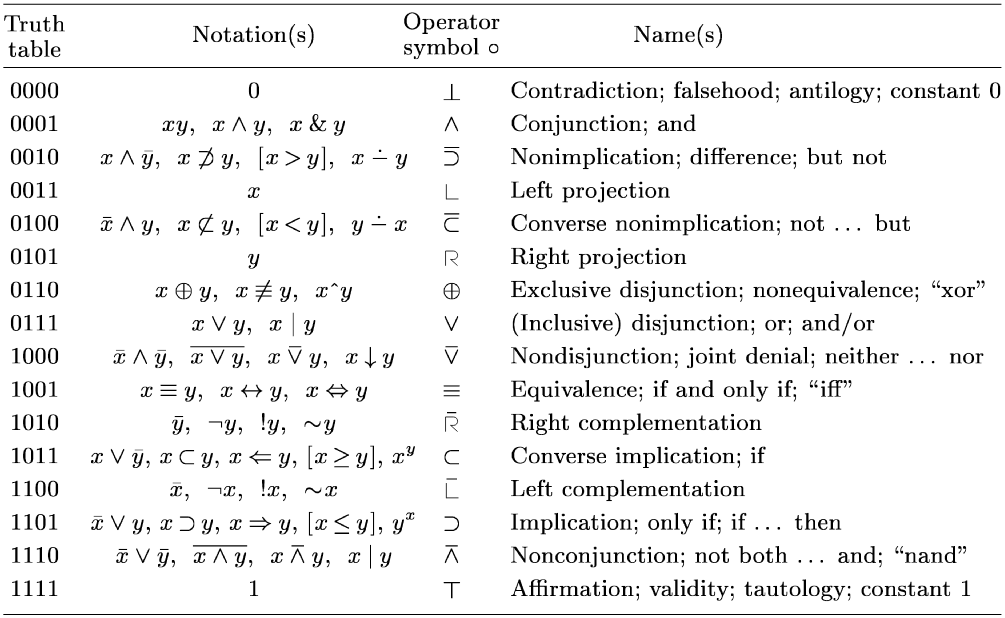
\includegraphics [width=5in]{TableOfPropositionalOperators}
   \caption{TableOfPropositionalOperators}
   \label{table:TableOfPropositionalOperators}
\end{table}

    \subsection {Boolean Expressions and Boolean Functions}
    \subsection {Identities of Boolean Algebra}
    \subsection {Principle of Duality}
Note the similarity of Table 1.1 and 2.1. This is no accident but instead is a fundamental point that is explored in more detail in the math course, Abstract Algebra. One fact that should be noted is the Principle of Duality.

    \subsection {Abstract Definition of a Boolean Algebra}

\section {Representing Boolean Functions}
    \subsection {Sum-of-Products Expansions}
    \subsection {Functional Completeness}
    
\section {Logic Gates}
combinational circuits versus sequential circuits
    \subsection {Combinations of Gates}
    \subsection {Adders}
    \subsection {Minimization of Circuits}
    \subsection {Karnaugh Maps and Quine-McCluskey Method}

Two meanings: one the notation used by Boole, the other the more general observation that this algebra is the same as for logic and sets. The general topic of other algebras is covered in a course on abstract algebra in the math department. 

Sum of Products form for Boolean Algebras
well formed formula
fundamental product
Algorithm for finding sum-of-products form
complete sum of products form, midterms, DNF

Homomorphism between Boolean Algebra and basic logic gates


                                                                                                  %%%%       GRAPHS           %%%

\chapter {Graph Theory}
vertices or nodes, edges (directed or undirected), head, tail, in-degree, out-degree, self-loop (reflexive), was covered in the chapter on functions.
Famous algorithms for graph traversal


\section {Graphs and Graph Models}
\begin{definition}
A \textit{graph} $G =(V,E)$ consistes of a non-empty set $V$ of \textit{vertices} or \textit{nodes} and $E$, a set of \textit{edges}. Each edge has either one or two vertices associated ith it, called its \textit{endpoints}. An edge is said to \textit{connect} its endpoints.
\end{definition}
\begin{notes}
The number of vertices does not need to be finite. But we will only discuss finite graphs in this outline.
\end{notes}

\begin {definition} [Simple Graph]
A graph in which each edge connects two different vertices and where no two edges connect the same pair of vertices is called a \textbf{simple graph}. The edge in a simple graph can be denoted by the set of vertices it connects.
\end{definition}

\begin {definition}[Multigraph]
Graphs that have multiple edges connecting the same vertices are called \textbf{multigraphs}. We say that each edge has a multiplicity of edges between the two vertices.
\end{definition}

\begin{definition}
A \textit{directed graph} (or \textit{digraph} $(V,E)$ consists of a nonempty set of vertices $V$ and a set of \textit{directed edges} or \textit{arcs} $E$. Each directed edge is associated with an ordereed pair of vertices. The directed edge associated with the ordered pair $(u,v)$ is said to start with $u$ and end at $v$. When presented in a picture, the directed edge has an arrow that starts at the vertex $u$ and ends at $v$. A directed graph may also have multiple directed edges.
\end{definition}

Graphs model a great many applications in software engineering. They include Acuaintanceship Graphs, Influence Graphs, The Hollywood Graph, Round-Robin Tournaments, Collaboration Graphs, Road Maps, Call Graphs, and the WWW.

\section {Graph Terminology and Special Types of Graphs}
\begin{definition}
Two vertices $u$ and $v$ in an undirected graph $G$ are called \textit{adjacent} (or \textit{neighbors} in $G$ if $u$ and $v$ are endpoints of an edge of $G$. If $e$ is associated with $\{u,v\}$, the edge $e$ is called \textit{incident with} the vertices $u$ and $v$. The edge $e$ is also said to \textit{connect u} and \textit{v}. The vertices $u$ and $v$ ar called \textit{endpoints} of an edge associated with $\{u,v\}$.
\end{definition}

\section {Representing Graphs and Graph Isomorphism}
\section {Connectivity}
\section {Euler and Hamilton Paths}
\section {Shortest Path Problem}
\section {Planar Graphs}
\section {Graph Coloring}

\newpage

                                                                                                %%%    TREES    %%%
\chapter {Trees}
Recursive def of trees, some famous algorithms for trees

\section {Applications of Trees}
\section {Tree Traversal}
\section {Spanning Trees}
\section {Minimum Spanning Trees}

\newpage

%%%   PROBABILITY   %%%
\chapter {Discrete Probability}
\section {An Introduction to Discrete Probability}
    \subsection {Finite Probability}
    \subsection {The Probability of Combinations of Events}
    \subsection {Probabilistic Reasoning}

\section {Probability Theory}
    \subsection {Assigning Probabilities}
    \subsection {Combinations of Events}
    \subsection {Conditional Probability}
    \subsection {Independence}
    \subsection {Bernoulli Trials and the Binomial Distrubution}
    \subsection {The Birthday Problem}
    \subsection {Monte Carlo Algorithms}
    \subsection {The Probabilistic Method}






Let p be the proposition that the sum of the first n odd numbers is n**2. How can we prove such a proposition? Here is the example of how inductive reasoning works. 

We can easily evaluate this proposition for small values of n and see that they are true. But since the set of input values is the set of natural numbers we cannot do this for all elements of the set. So we observe this, let us assume that this proposition is true for some value k which is bigger than any value we evaluated manually. If we can prove that the statement MUST be true for the next value, the successor of k, k+1, then we have proven that it must be true for ALL values of n drawn from the natural numbers since we know it is true for the small values and we can continually apply the reasoning that got us from k to k+1 as many times as we need to give us all the values to infinity.

So first we introduce the inductive hypothesis, that it is true for some k:
Assume that the first k odd numbers sum to k**2. Now we have the proof obligation to prove that with that assumption that this MUST be true for k+1, that is, the sum of the first k+1 odd numbers will give us (k+1)**2. This requires some clever algebra but nothing you can't follow:

the first k odd number sum to k**2
Sigma(i=0 to k, 2i+1) = Sigma(i=1 to k-1, 2i+1) = k**2
which is equivalent to 
1+3+5+ ... +2(k-1) = k**2
we add 2(k+1) to both sides of the equation giving
1+3+5+ ... +2(k-1)+2(k+1) = (k+1)**2 = (k**2 + 2k + 1)=k**2 + (2k+1)
Using the premise, we rewrite the LHS
1+3+5+ ... +2(k-1)  + 2(k+1) = k**2 + 2(k+1)= k**2 + 2k + 1
showing the left and RHS of the equation are equal QED.

The general principle of weak form of mathematical induction is
First, show the proposition is true for one small element from the input.
Show that IF the proposition is true for some arbitrary k, that it MUST also be true for the next value after k, k+1. 
After both parts are proven, you have proven for all value from N.

CAUTION: The inductive assumption looks similar to the thing to be proven but you may not use that in the argument. You must use an arbitrary value k, and then prove that it must also be true for k+1 without again stating the assumption. To do so is the famous logical fallacy of assuming the antecedent or begging the question. This is a common error in inductive proofs.

There are a set of proofs that can be solved inductively but require that more than one small value be proven. This leads to the stronger form of inductive reasoning. In the strong form, you must prove that the proposition holds for some small number of values.

Open Form versus Closed Form Solutions
Note that we have proved an equivalence between two expressions, the sum of the first n odd numbers and the expression n**2. The first form has the implied algorithm of summing the first n odd integers, something that is of O(n) while the second has O(1). We call the first version an open form solution while we call the second a closed form solution. The computational advantage is obvious.

\newpage




           %%% COMPUTATION and FORMAL LANGUAGES  %%%
                                                                 
% This chapter can be skipped for programs that require a Theory of Computation Course that does not have a prerequisite
(Excluded from UCD course offerings)
\chapter {Computation}
Association between Automata, Grammar, Language. Difference between syntax and semantics in natural language. Object first or object last in natural language. 

\section {Languages and Grammars}
We saw that the notation $A_*$ designates all the possible strings that can be constructed from the set $A$. When the set A contains symbols that are distinguishable from each other we call that set an $\textit{alphabet}$ and refer to it with the greek letter $\Sigma$. Since there is no ambiguity between the strings $(a_1,a_2, \dots a_n)$ and $a_1a_2a_3 \dots a_n$ for strings of length $n$, we adopt this notation for string sequences. For short strings then
$$(w,o,r,d) = word$$
We call such strings words, the symbols from the alphabet lettersand the finite sequences in $\Sigma_*$ as the strings or words generated by the letters of $\Sigma$.

Alphabet, Words
Operations on words: concatenation
Formal Definition of Language
Operations on Languages
    \subsection {Phrase-Structured Grammars}
Regular Expressions, Regular Languages
Generative Grammars, Rules of Production
    \subsection {Context Free and Context Sensitive Grammars}
    \subsection {Regular Languages and their Notation}
    \subsection {Derivation Trees}
    parsing
    \subsection {Backus-Naur Form}
    
\section {Finite State Machines}
States, State Transition, Finite State Automata
    \subsection {FSM with no output}
        \subsubsection {Set of Strings}
        \subsubsection {Finite-State Automata}
        Def 3: A \textit{finite-state automata} $M=(S,I,f,s_0,F)$ consists of a finite set $S$ of \textit{states}, a finite \textit{input alphabet} $I$, a \textit{transition function} $f$ that assigns a next state to every pair of state and input (so that $f:S \times I \rightarrow S$, an \textit{initial} or \textit{start state} $s_0$, and a subset $F$ of $S$ consisting of \textit{final} (or \textit{accepting states}.
        
        \subsubsection {Language Recognition by FSA}
        \subsubsection {Non-deterministic FSA}
        
    \subsection {FSM with output}
    Mealy and Moore machines
    
\section {Language Recognition}
    \subsection {Regular Sets}
    \subsection {Kleene's Theorem}
    \subsection {Regular Sets and Regular Grammars}
    \subsection {Beyond Regular Languages and FSMs}
A later class will explore grammars beyond regular grammars, the languages they generate and the automata that recognize them.




\newpage


  
%%%%%%%%%%%%%%%%%%%%%%%%%%%%%%
\end{document}
